\section*{Results}
\label{Results} 

Table~\ref{table1} displays the results from our model. As expected, we find support for hypothesis one, which states that as the number of sender states increases for any given sanction case, the time to compliance will decrease. We also find support for our second hypothesis, that more proximate relationships between sender and recievers result in quicker compliance by the target state. However, support for this hypothesis is limited to the type of relationship or proximity that is measured. Our findings reveal that distance and religion are influential for predicting compliance. This suggests that target states are most sensitive to sanctions by those states whose are both neighbors and share cultural similarities. We also find support for hypothesis three, that states are more likely to comply to one sanction when they are simultaneously facing a number of others. 

We control for the prominent idea from the literature that domestic factors influence sanction compliance. We find that while our measure of internal stabiity does not play a role, %we need to define this variable somewhere. 
domestic institutions do matter. Interestingly, we find little support for trade and alliances having an influence on compliance. 
Because it is difficult to interpret the effect of point estimates on the hazard function in tabular form, we present a graphical interpretation below. 

% latex table generated in R 3.1.0 by xtable 1.7-3 package
% Sat Aug  2 12:32:14 2014
\begin{table}[ht]
\centering
{\normalsize
\begin{tabular}{lccc}
 Variable & Model 1 & Model 2 & Model 3 \\ 
  \hline
\hline
Compliance Reciprocity$_{j,t-1}$ &  &  & $0.212^{\ast\ast}$ \\ 
   &  &  & (0.063) \\ 
  Sanction Reciprocity$_{j,t-1}$ &  &  & $-0.103^{\ast\ast}$ \\ 
   &  &  & (0.033) \\ 
   \hline
Number of Senders$_{j,t}$ &  & $0.255^{\ast\ast}$ & $0.234^{\ast\ast}$ \\ 
   &  & (0.062) & (0.062) \\ 
  Distance$_{j,t}$ &  & $0.531^{\ast\ast}$ & $0.497^{\ast\ast}$ \\ 
   &  & (0.183) & (0.187) \\ 
  Trade$_{j,t}$ &  & $16.795^{\ast}$ & $16.106^{\ast}$ \\ 
   &  & (9.393) & (9.398) \\ 
  Ally$_{j,t}$ &  & 0.029 & 0.096 \\ 
   &  & (0.159) & (0.164) \\ 
   \hline
Polity$_{i,t-1}$ & $-0.029^{\ast}$ & -0.015 & -0.022 \\ 
   & (0.016) & (0.017) & (0.017) \\ 
  Ln(GDP per capita)$_{i,t-1}$ & -0.088 & -0.08 & -0.03 \\ 
   & (0.065) & (0.07) & (0.073) \\ 
  GDP Growth$_{i,t-1}$ & 0.011 & 0.02 & 0.015 \\ 
   & (0.018) & (0.019) & (0.019) \\ 
  Population$_{i,t-1}$ & $-0.172^{\ast\ast}$ & $-0.16^{\ast\ast}$ & $-0.102^{\ast\ast}$ \\ 
   & (0.039) & (0.043) & (0.05) \\ 
  Internal Conflict$_{i,t-1}$ & 0.001 & 0.004 & -0.001 \\ 
   & (0.017) & (0.017) & (0.017) \\ 
   \hline
n & 6517 & 6483 & 6483 \\ 
  Events & 191 & 190 & 190 \\ 
  Likelihood ratio test & 36.91 (0) & 59.55 (0) & 70.76 (0) \\ 
   \hline
\hline
\end{tabular}
}
\caption{Duration model with time varying covariates estimated using Cox Proportional Hazards. Standard errors in parentheses. $^{**}$ and $^{*}$ indicate significance at $p< 0.05 $ and $p< 0.10 $, respectively.} 
\label{tab:regResults}
\end{table}


\begin{figure}[ht]
	\centering
	\caption{Survival Probability by Number of Senders in a Sanction Case}
	% \includegraphics[width=1\textwidth]{nosSurv}
	\resizebox{1\textwidth}{!}{% Created by tikzDevice version 0.8.1 on 2015-05-16 17:34:47
% !TEX encoding = UTF-8 Unicode
\begin{tikzpicture}[x=1pt,y=1pt]
\definecolor{fillColor}{RGB}{255,255,255}
\path[use as bounding box,fill=fillColor,fill opacity=0.00] (0,0) rectangle (433.62,289.08);
\begin{scope}
\path[clip] (  0.00,  0.00) rectangle (433.62,289.08);
\definecolor{drawColor}{RGB}{0,0,0}

\path[draw=drawColor,line width= 0.4pt,line join=round,line cap=round] ( 49.20, 61.20) -- (408.42, 61.20);

\path[draw=drawColor,line width= 0.4pt,line join=round,line cap=round] ( 49.20, 61.20) -- ( 49.20, 55.20);

\path[draw=drawColor,line width= 0.4pt,line join=round,line cap=round] (109.07, 61.20) -- (109.07, 55.20);

\path[draw=drawColor,line width= 0.4pt,line join=round,line cap=round] (168.94, 61.20) -- (168.94, 55.20);

\path[draw=drawColor,line width= 0.4pt,line join=round,line cap=round] (228.81, 61.20) -- (228.81, 55.20);

\path[draw=drawColor,line width= 0.4pt,line join=round,line cap=round] (288.68, 61.20) -- (288.68, 55.20);

\path[draw=drawColor,line width= 0.4pt,line join=round,line cap=round] (348.55, 61.20) -- (348.55, 55.20);

\path[draw=drawColor,line width= 0.4pt,line join=round,line cap=round] (408.42, 61.20) -- (408.42, 55.20);

\node[text=drawColor,anchor=base,inner sep=0pt, outer sep=0pt, scale=  1.00] at ( 49.20, 39.60) {0};

\node[text=drawColor,anchor=base,inner sep=0pt, outer sep=0pt, scale=  1.00] at (109.07, 39.60) {5};

\node[text=drawColor,anchor=base,inner sep=0pt, outer sep=0pt, scale=  1.00] at (168.94, 39.60) {10};

\node[text=drawColor,anchor=base,inner sep=0pt, outer sep=0pt, scale=  1.00] at (228.81, 39.60) {15};

\node[text=drawColor,anchor=base,inner sep=0pt, outer sep=0pt, scale=  1.00] at (288.68, 39.60) {20};

\node[text=drawColor,anchor=base,inner sep=0pt, outer sep=0pt, scale=  1.00] at (348.55, 39.60) {25};

\node[text=drawColor,anchor=base,inner sep=0pt, outer sep=0pt, scale=  1.00] at (408.42, 39.60) {30};

\path[draw=drawColor,line width= 0.4pt,line join=round,line cap=round] ( 49.20, 67.82) -- ( 49.20,233.26);

\path[draw=drawColor,line width= 0.4pt,line join=round,line cap=round] ( 49.20, 67.82) -- ( 43.20, 67.82);

\path[draw=drawColor,line width= 0.4pt,line join=round,line cap=round] ( 49.20,109.18) -- ( 43.20,109.18);

\path[draw=drawColor,line width= 0.4pt,line join=round,line cap=round] ( 49.20,150.54) -- ( 43.20,150.54);

\path[draw=drawColor,line width= 0.4pt,line join=round,line cap=round] ( 49.20,191.90) -- ( 43.20,191.90);

\path[draw=drawColor,line width= 0.4pt,line join=round,line cap=round] ( 49.20,233.26) -- ( 43.20,233.26);

\node[text=drawColor,anchor=base east,inner sep=0pt, outer sep=0pt, scale=  1.00] at ( 37.20, 64.37) {0.2};

\node[text=drawColor,anchor=base east,inner sep=0pt, outer sep=0pt, scale=  1.00] at ( 37.20,105.74) {0.4};

\node[text=drawColor,anchor=base east,inner sep=0pt, outer sep=0pt, scale=  1.00] at ( 37.20,147.10) {0.6};

\node[text=drawColor,anchor=base east,inner sep=0pt, outer sep=0pt, scale=  1.00] at ( 37.20,188.46) {0.8};

\node[text=drawColor,anchor=base east,inner sep=0pt, outer sep=0pt, scale=  1.00] at ( 37.20,229.82) {1.0};
\end{scope}
\begin{scope}
\path[clip] (  0.00,  0.00) rectangle (433.62,289.08);
\definecolor{drawColor}{RGB}{0,0,0}

\node[text=drawColor,anchor=base,inner sep=0pt, outer sep=0pt, scale=  1.00] at (228.81, 15.60) {Time (Years)};

\node[text=drawColor,rotate= 90.00,anchor=base,inner sep=0pt, outer sep=0pt, scale=  1.00] at ( 10.80,150.54) {Survival Probability};
\end{scope}
\begin{scope}
\path[clip] ( 49.20, 61.20) rectangle (408.42,239.88);
\definecolor{drawColor}{RGB}{169,169,169}

\path[draw=drawColor,line width= 0.4pt,line join=round,line cap=round] ( 49.20,233.26) --
	( 61.17,233.26) --
	( 61.17,229.01) --
	( 73.15,229.01) --
	( 73.15,224.14) --
	( 85.12,224.14) --
	( 85.12,218.85) --
	( 97.10,218.85) --
	( 97.10,215.94) --
	(109.07,215.94) --
	(109.07,214.09) --
	(121.04,214.09) --
	(121.04,213.30) --
	(133.02,213.30) --
	(133.02,212.92) --
	(144.99,212.92) --
	(144.99,212.50) --
	(156.97,212.50) --
	(156.97,212.03) --
	(168.94,212.03) --
	(168.94,211.56) --
	(180.91,211.56) --
	(180.91,211.05) --
	(204.86,211.05) --
	(204.86,210.45) --
	(216.84,210.45) --
	(216.84,209.80) --
	(252.76,209.80) --
	(252.76,208.69) --
	(264.73,208.69) --
	(264.73,206.89) --
	(288.68,206.89) --
	(288.68,203.45) --
	(300.65,203.45) --
	(300.65,199.35) --
	(336.58,199.35) --
	(336.58,195.48) --
	(433.62,195.48);

\path[draw=drawColor,line width= 0.4pt,line join=round,line cap=round] ( 57.99,229.01) -- ( 64.36,229.01);

\path[draw=drawColor,line width= 0.4pt,line join=round,line cap=round] ( 61.17,225.83) -- ( 61.17,232.19);

\path[draw=drawColor,line width= 0.4pt,line join=round,line cap=round] ( 69.97,224.14) -- ( 76.33,224.14);

\path[draw=drawColor,line width= 0.4pt,line join=round,line cap=round] ( 73.15,220.95) -- ( 73.15,227.32);

\path[draw=drawColor,line width= 0.4pt,line join=round,line cap=round] ( 81.94,218.85) -- ( 88.30,218.85);

\path[draw=drawColor,line width= 0.4pt,line join=round,line cap=round] ( 85.12,215.67) -- ( 85.12,222.03);

\path[draw=drawColor,line width= 0.4pt,line join=round,line cap=round] ( 93.91,215.94) -- (100.28,215.94);

\path[draw=drawColor,line width= 0.4pt,line join=round,line cap=round] ( 97.10,212.76) -- ( 97.10,219.12);

\path[draw=drawColor,line width= 0.4pt,line join=round,line cap=round] (105.89,214.09) -- (112.25,214.09);

\path[draw=drawColor,line width= 0.4pt,line join=round,line cap=round] (109.07,210.91) -- (109.07,217.27);

\path[draw=drawColor,line width= 0.4pt,line join=round,line cap=round] (117.86,213.30) -- (124.23,213.30);

\path[draw=drawColor,line width= 0.4pt,line join=round,line cap=round] (121.04,210.12) -- (121.04,216.49);

\path[draw=drawColor,line width= 0.4pt,line join=round,line cap=round] (129.84,212.92) -- (136.20,212.92);

\path[draw=drawColor,line width= 0.4pt,line join=round,line cap=round] (133.02,209.74) -- (133.02,216.10);

\path[draw=drawColor,line width= 0.4pt,line join=round,line cap=round] (141.81,212.50) -- (148.17,212.50);

\path[draw=drawColor,line width= 0.4pt,line join=round,line cap=round] (144.99,209.32) -- (144.99,215.68);

\path[draw=drawColor,line width= 0.4pt,line join=round,line cap=round] (153.78,212.03) -- (160.15,212.03);

\path[draw=drawColor,line width= 0.4pt,line join=round,line cap=round] (156.97,208.85) -- (156.97,215.21);

\path[draw=drawColor,line width= 0.4pt,line join=round,line cap=round] (165.76,211.56) -- (172.12,211.56);

\path[draw=drawColor,line width= 0.4pt,line join=round,line cap=round] (168.94,208.38) -- (168.94,214.74);

\path[draw=drawColor,line width= 0.4pt,line join=round,line cap=round] (177.73,211.05) -- (184.10,211.05);

\path[draw=drawColor,line width= 0.4pt,line join=round,line cap=round] (180.91,207.87) -- (180.91,214.24);

\path[draw=drawColor,line width= 0.4pt,line join=round,line cap=round] (189.71,211.05) -- (196.07,211.05);

\path[draw=drawColor,line width= 0.4pt,line join=round,line cap=round] (192.89,207.87) -- (192.89,214.24);

\path[draw=drawColor,line width= 0.4pt,line join=round,line cap=round] (201.68,210.45) -- (208.04,210.45);

\path[draw=drawColor,line width= 0.4pt,line join=round,line cap=round] (204.86,207.27) -- (204.86,213.63);

\path[draw=drawColor,line width= 0.4pt,line join=round,line cap=round] (213.65,209.80) -- (220.02,209.80);

\path[draw=drawColor,line width= 0.4pt,line join=round,line cap=round] (216.84,206.62) -- (216.84,212.98);

\path[draw=drawColor,line width= 0.4pt,line join=round,line cap=round] (225.63,209.80) -- (231.99,209.80);

\path[draw=drawColor,line width= 0.4pt,line join=round,line cap=round] (228.81,206.62) -- (228.81,212.98);

\path[draw=drawColor,line width= 0.4pt,line join=round,line cap=round] (237.60,209.80) -- (243.97,209.80);

\path[draw=drawColor,line width= 0.4pt,line join=round,line cap=round] (240.78,206.62) -- (240.78,212.98);

\path[draw=drawColor,line width= 0.4pt,line join=round,line cap=round] (249.58,208.69) -- (255.94,208.69);

\path[draw=drawColor,line width= 0.4pt,line join=round,line cap=round] (252.76,205.51) -- (252.76,211.87);

\path[draw=drawColor,line width= 0.4pt,line join=round,line cap=round] (261.55,206.89) -- (267.91,206.89);

\path[draw=drawColor,line width= 0.4pt,line join=round,line cap=round] (264.73,203.71) -- (264.73,210.08);

\path[draw=drawColor,line width= 0.4pt,line join=round,line cap=round] (273.52,206.89) -- (279.89,206.89);

\path[draw=drawColor,line width= 0.4pt,line join=round,line cap=round] (276.71,203.71) -- (276.71,210.08);

\path[draw=drawColor,line width= 0.4pt,line join=round,line cap=round] (285.50,203.45) -- (291.86,203.45);

\path[draw=drawColor,line width= 0.4pt,line join=round,line cap=round] (288.68,200.27) -- (288.68,206.63);

\path[draw=drawColor,line width= 0.4pt,line join=round,line cap=round] (297.47,199.35) -- (303.84,199.35);

\path[draw=drawColor,line width= 0.4pt,line join=round,line cap=round] (300.65,196.17) -- (300.65,202.53);

\path[draw=drawColor,line width= 0.4pt,line join=round,line cap=round] (309.45,199.35) -- (315.81,199.35);

\path[draw=drawColor,line width= 0.4pt,line join=round,line cap=round] (312.63,196.17) -- (312.63,202.53);

\path[draw=drawColor,line width= 0.4pt,line join=round,line cap=round] (321.42,199.35) -- (327.78,199.35);

\path[draw=drawColor,line width= 0.4pt,line join=round,line cap=round] (324.60,196.17) -- (324.60,202.53);

\path[draw=drawColor,line width= 0.4pt,line join=round,line cap=round] (333.39,195.48) -- (339.76,195.48);

\path[draw=drawColor,line width= 0.4pt,line join=round,line cap=round] (336.58,192.30) -- (336.58,198.66);

\path[draw=drawColor,line width= 0.4pt,line join=round,line cap=round] (345.37,195.48) -- (351.73,195.48);

\path[draw=drawColor,line width= 0.4pt,line join=round,line cap=round] (348.55,192.30) -- (348.55,198.66);

\path[draw=drawColor,line width= 0.4pt,line join=round,line cap=round] (357.34,195.48) -- (363.71,195.48);

\path[draw=drawColor,line width= 0.4pt,line join=round,line cap=round] (360.52,192.30) -- (360.52,198.66);

\path[draw=drawColor,line width= 0.4pt,line join=round,line cap=round] (369.32,195.48) -- (375.68,195.48);

\path[draw=drawColor,line width= 0.4pt,line join=round,line cap=round] (372.50,192.30) -- (372.50,198.66);

\path[draw=drawColor,line width= 0.4pt,line join=round,line cap=round] (381.29,195.48) -- (387.65,195.48);

\path[draw=drawColor,line width= 0.4pt,line join=round,line cap=round] (384.47,192.30) -- (384.47,198.66);

\path[draw=drawColor,line width= 0.4pt,line join=round,line cap=round] (393.26,195.48) -- (399.63,195.48);

\path[draw=drawColor,line width= 0.4pt,line join=round,line cap=round] (396.45,192.30) -- (396.45,198.66);

\path[draw=drawColor,line width= 0.4pt,line join=round,line cap=round] (405.24,195.48) -- (411.60,195.48);

\path[draw=drawColor,line width= 0.4pt,line join=round,line cap=round] (408.42,192.30) -- (408.42,198.66);

\path[draw=drawColor,line width= 0.4pt,line join=round,line cap=round] (417.21,195.48) -- (423.58,195.48);

\path[draw=drawColor,line width= 0.4pt,line join=round,line cap=round] (420.39,192.30) -- (420.39,198.66);

\path[draw=drawColor,line width= 0.4pt,line join=round,line cap=round] (429.19,195.48) -- (433.62,195.48);

\path[draw=drawColor,line width= 0.4pt,line join=round,line cap=round] (432.37,192.30) -- (432.37,198.66);

\path[draw=drawColor,line width= 0.4pt,dash pattern=on 4pt off 4pt ,line join=round,line cap=round] ( 49.20,233.26) --
	( 61.17,233.26) --
	( 61.17,226.45) --
	( 73.15,226.45) --
	( 73.15,220.05) --
	( 85.12,220.05) --
	( 85.12,213.23) --
	( 97.10,213.23) --
	( 97.10,209.55) --
	(109.07,209.55) --
	(109.07,207.24) --
	(121.04,207.24) --
	(121.04,206.27) --
	(133.02,206.27) --
	(133.02,205.79) --
	(144.99,205.79) --
	(144.99,205.27) --
	(156.97,205.27) --
	(156.97,204.69) --
	(168.94,204.69) --
	(168.94,204.11) --
	(180.91,204.11) --
	(180.91,203.48) --
	(204.86,203.48) --
	(204.86,202.74) --
	(216.84,202.74) --
	(216.84,201.94) --
	(252.76,201.94) --
	(252.76,200.45) --
	(264.73,200.45) --
	(264.73,197.84) --
	(288.68,197.84) --
	(288.68,192.13) --
	(300.65,192.13) --
	(300.65,185.35) --
	(336.58,185.35) --
	(336.58,179.19) --
	(433.62,179.19);

\path[draw=drawColor,line width= 0.4pt,dash pattern=on 4pt off 4pt ,line join=round,line cap=round] ( 49.20,233.26) --
	( 61.17,233.26) --
	( 61.17,231.60) --
	( 73.15,231.60) --
	( 73.15,228.31) --
	( 85.12,228.31) --
	( 85.12,224.64) --
	( 97.10,224.64) --
	( 97.10,222.56) --
	(109.07,222.56) --
	(109.07,221.20) --
	(121.04,221.20) --
	(121.04,220.62) --
	(133.02,220.62) --
	(133.02,220.34) --
	(144.99,220.34) --
	(144.99,220.02) --
	(156.97,220.02) --
	(156.97,219.67) --
	(168.94,219.67) --
	(168.94,219.32) --
	(180.91,219.32) --
	(180.91,218.95) --
	(204.86,218.95) --
	(204.86,218.50) --
	(216.84,218.50) --
	(216.84,218.02) --
	(252.76,218.02) --
	(252.76,217.32) --
	(264.73,217.32) --
	(264.73,216.43) --
	(288.68,216.43) --
	(288.68,215.55) --
	(300.65,215.55) --
	(300.65,214.59) --
	(336.58,214.59) --
	(336.58,213.50) --
	(433.62,213.50);
\definecolor{drawColor}{RGB}{0,0,0}

\path[draw=drawColor,line width= 0.4pt,line join=round,line cap=round] ( 49.20,233.26) --
	( 61.17,233.26) --
	( 61.17,216.17) --
	( 73.15,216.17) --
	( 73.15,197.92) --
	( 85.12,197.92) --
	( 85.12,179.68) --
	( 97.10,179.68) --
	( 97.10,170.29) --
	(109.07,170.29) --
	(109.07,164.54) --
	(121.04,164.54) --
	(121.04,162.15) --
	(133.02,162.15) --
	(133.02,161.00) --
	(144.99,161.00) --
	(144.99,159.74) --
	(156.97,159.74) --
	(156.97,158.35) --
	(168.94,158.35) --
	(168.94,156.97) --
	(180.91,156.97) --
	(180.91,155.49) --
	(204.86,155.49) --
	(204.86,153.75) --
	(216.84,153.75) --
	(216.84,151.90) --
	(252.76,151.90) --
	(252.76,148.77) --
	(264.73,148.77) --
	(264.73,143.84) --
	(288.68,143.84) --
	(288.68,134.82) --
	(300.65,134.82) --
	(300.65,124.77) --
	(336.58,124.77) --
	(336.58,115.95) --
	(433.62,115.95);

\path[draw=drawColor,line width= 0.4pt,line join=round,line cap=round] ( 57.99,216.17) -- ( 64.36,216.17);

\path[draw=drawColor,line width= 0.4pt,line join=round,line cap=round] ( 61.17,212.99) -- ( 61.17,219.35);

\path[draw=drawColor,line width= 0.4pt,line join=round,line cap=round] ( 69.97,197.92) -- ( 76.33,197.92);

\path[draw=drawColor,line width= 0.4pt,line join=round,line cap=round] ( 73.15,194.74) -- ( 73.15,201.10);

\path[draw=drawColor,line width= 0.4pt,line join=round,line cap=round] ( 81.94,179.68) -- ( 88.30,179.68);

\path[draw=drawColor,line width= 0.4pt,line join=round,line cap=round] ( 85.12,176.50) -- ( 85.12,182.86);

\path[draw=drawColor,line width= 0.4pt,line join=round,line cap=round] ( 93.91,170.29) -- (100.28,170.29);

\path[draw=drawColor,line width= 0.4pt,line join=round,line cap=round] ( 97.10,167.10) -- ( 97.10,173.47);

\path[draw=drawColor,line width= 0.4pt,line join=round,line cap=round] (105.89,164.54) -- (112.25,164.54);

\path[draw=drawColor,line width= 0.4pt,line join=round,line cap=round] (109.07,161.36) -- (109.07,167.72);

\path[draw=drawColor,line width= 0.4pt,line join=round,line cap=round] (117.86,162.15) -- (124.23,162.15);

\path[draw=drawColor,line width= 0.4pt,line join=round,line cap=round] (121.04,158.97) -- (121.04,165.33);

\path[draw=drawColor,line width= 0.4pt,line join=round,line cap=round] (129.84,161.00) -- (136.20,161.00);

\path[draw=drawColor,line width= 0.4pt,line join=round,line cap=round] (133.02,157.82) -- (133.02,164.18);

\path[draw=drawColor,line width= 0.4pt,line join=round,line cap=round] (141.81,159.74) -- (148.17,159.74);

\path[draw=drawColor,line width= 0.4pt,line join=round,line cap=round] (144.99,156.55) -- (144.99,162.92);

\path[draw=drawColor,line width= 0.4pt,line join=round,line cap=round] (153.78,158.35) -- (160.15,158.35);

\path[draw=drawColor,line width= 0.4pt,line join=round,line cap=round] (156.97,155.17) -- (156.97,161.54);

\path[draw=drawColor,line width= 0.4pt,line join=round,line cap=round] (165.76,156.97) -- (172.12,156.97);

\path[draw=drawColor,line width= 0.4pt,line join=round,line cap=round] (168.94,153.79) -- (168.94,160.15);

\path[draw=drawColor,line width= 0.4pt,line join=round,line cap=round] (177.73,155.49) -- (184.10,155.49);

\path[draw=drawColor,line width= 0.4pt,line join=round,line cap=round] (180.91,152.31) -- (180.91,158.68);

\path[draw=drawColor,line width= 0.4pt,line join=round,line cap=round] (189.71,155.49) -- (196.07,155.49);

\path[draw=drawColor,line width= 0.4pt,line join=round,line cap=round] (192.89,152.31) -- (192.89,158.68);

\path[draw=drawColor,line width= 0.4pt,line join=round,line cap=round] (201.68,153.75) -- (208.04,153.75);

\path[draw=drawColor,line width= 0.4pt,line join=round,line cap=round] (204.86,150.57) -- (204.86,156.93);

\path[draw=drawColor,line width= 0.4pt,line join=round,line cap=round] (213.65,151.90) -- (220.02,151.90);

\path[draw=drawColor,line width= 0.4pt,line join=round,line cap=round] (216.84,148.72) -- (216.84,155.08);

\path[draw=drawColor,line width= 0.4pt,line join=round,line cap=round] (225.63,151.90) -- (231.99,151.90);

\path[draw=drawColor,line width= 0.4pt,line join=round,line cap=round] (228.81,148.72) -- (228.81,155.08);

\path[draw=drawColor,line width= 0.4pt,line join=round,line cap=round] (237.60,151.90) -- (243.97,151.90);

\path[draw=drawColor,line width= 0.4pt,line join=round,line cap=round] (240.78,148.72) -- (240.78,155.08);

\path[draw=drawColor,line width= 0.4pt,line join=round,line cap=round] (249.58,148.77) -- (255.94,148.77);

\path[draw=drawColor,line width= 0.4pt,line join=round,line cap=round] (252.76,145.59) -- (252.76,151.95);

\path[draw=drawColor,line width= 0.4pt,line join=round,line cap=round] (261.55,143.84) -- (267.91,143.84);

\path[draw=drawColor,line width= 0.4pt,line join=round,line cap=round] (264.73,140.66) -- (264.73,147.02);

\path[draw=drawColor,line width= 0.4pt,line join=round,line cap=round] (273.52,143.84) -- (279.89,143.84);

\path[draw=drawColor,line width= 0.4pt,line join=round,line cap=round] (276.71,140.66) -- (276.71,147.02);

\path[draw=drawColor,line width= 0.4pt,line join=round,line cap=round] (285.50,134.82) -- (291.86,134.82);

\path[draw=drawColor,line width= 0.4pt,line join=round,line cap=round] (288.68,131.64) -- (288.68,138.01);

\path[draw=drawColor,line width= 0.4pt,line join=round,line cap=round] (297.47,124.77) -- (303.84,124.77);

\path[draw=drawColor,line width= 0.4pt,line join=round,line cap=round] (300.65,121.59) -- (300.65,127.95);

\path[draw=drawColor,line width= 0.4pt,line join=round,line cap=round] (309.45,124.77) -- (315.81,124.77);

\path[draw=drawColor,line width= 0.4pt,line join=round,line cap=round] (312.63,121.59) -- (312.63,127.95);

\path[draw=drawColor,line width= 0.4pt,line join=round,line cap=round] (321.42,124.77) -- (327.78,124.77);

\path[draw=drawColor,line width= 0.4pt,line join=round,line cap=round] (324.60,121.59) -- (324.60,127.95);

\path[draw=drawColor,line width= 0.4pt,line join=round,line cap=round] (333.39,115.95) -- (339.76,115.95);

\path[draw=drawColor,line width= 0.4pt,line join=round,line cap=round] (336.58,112.77) -- (336.58,119.13);

\path[draw=drawColor,line width= 0.4pt,line join=round,line cap=round] (345.37,115.95) -- (351.73,115.95);

\path[draw=drawColor,line width= 0.4pt,line join=round,line cap=round] (348.55,112.77) -- (348.55,119.13);

\path[draw=drawColor,line width= 0.4pt,line join=round,line cap=round] (357.34,115.95) -- (363.71,115.95);

\path[draw=drawColor,line width= 0.4pt,line join=round,line cap=round] (360.52,112.77) -- (360.52,119.13);

\path[draw=drawColor,line width= 0.4pt,line join=round,line cap=round] (369.32,115.95) -- (375.68,115.95);

\path[draw=drawColor,line width= 0.4pt,line join=round,line cap=round] (372.50,112.77) -- (372.50,119.13);

\path[draw=drawColor,line width= 0.4pt,line join=round,line cap=round] (381.29,115.95) -- (387.65,115.95);

\path[draw=drawColor,line width= 0.4pt,line join=round,line cap=round] (384.47,112.77) -- (384.47,119.13);

\path[draw=drawColor,line width= 0.4pt,line join=round,line cap=round] (393.26,115.95) -- (399.63,115.95);

\path[draw=drawColor,line width= 0.4pt,line join=round,line cap=round] (396.45,112.77) -- (396.45,119.13);

\path[draw=drawColor,line width= 0.4pt,line join=round,line cap=round] (405.24,115.95) -- (411.60,115.95);

\path[draw=drawColor,line width= 0.4pt,line join=round,line cap=round] (408.42,112.77) -- (408.42,119.13);

\path[draw=drawColor,line width= 0.4pt,line join=round,line cap=round] (417.21,115.95) -- (423.58,115.95);

\path[draw=drawColor,line width= 0.4pt,line join=round,line cap=round] (420.39,112.77) -- (420.39,119.13);

\path[draw=drawColor,line width= 0.4pt,line join=round,line cap=round] (429.19,115.95) -- (433.62,115.95);

\path[draw=drawColor,line width= 0.4pt,line join=round,line cap=round] (432.37,112.77) -- (432.37,119.13);

\path[draw=drawColor,line width= 0.4pt,dash pattern=on 4pt off 4pt ,line join=round,line cap=round] ( 49.20,233.26) --
	( 61.17,233.26) --
	( 61.17,203.55) --
	( 73.15,203.55) --
	( 73.15,177.09) --
	( 85.12,177.09) --
	( 85.12,152.36) --
	( 97.10,152.36) --
	( 97.10,140.23) --
	(109.07,140.23) --
	(109.07,132.99) --
	(121.04,132.99) --
	(121.04,130.06) --
	(133.02,130.06) --
	(133.02,128.64) --
	(144.99,128.64) --
	(144.99,127.09) --
	(156.97,127.09) --
	(156.97,125.40) --
	(168.94,125.40) --
	(168.94,123.71) --
	(180.91,123.71) --
	(180.91,121.92) --
	(204.86,121.92) --
	(204.86,119.84) --
	(216.84,119.84) --
	(216.84,117.64) --
	(252.76,117.64) --
	(252.76,113.86) --
	(264.73,113.86) --
	(264.73,107.91) --
	(288.68,107.91) --
	(288.68, 97.06) --
	(300.65, 97.06) --
	(300.65, 86.04) --
	(336.58, 86.04) --
	(336.58, 77.65) --
	(433.62, 77.65);

\path[draw=drawColor,line width= 0.4pt,dash pattern=on 4pt off 4pt ,line join=round,line cap=round] ( 49.20,233.26) --
	( 61.17,233.26) --
	( 61.17,229.69) --
	( 73.15,229.69) --
	( 73.15,221.63) --
	( 85.12,221.63) --
	( 85.12,212.93) --
	( 97.10,212.93) --
	( 97.10,208.28) --
	(109.07,208.28) --
	(109.07,205.43) --
	(121.04,205.43) --
	(121.04,204.18) --
	(133.02,204.18) --
	(133.02,203.61) --
	(144.99,203.61) --
	(144.99,202.96) --
	(156.97,202.96) --
	(156.97,202.29) --
	(168.94,202.29) --
	(168.94,201.60) --
	(180.91,201.60) --
	(180.91,200.88) --
	(204.86,200.88) --
	(204.86,199.97) --
	(216.84,199.97) --
	(216.84,199.03) --
	(252.76,199.03) --
	(252.76,197.62) --
	(264.73,197.62) --
	(264.73,195.63) --
	(288.68,195.63) --
	(288.68,192.77) --
	(300.65,192.77) --
	(300.65,188.69) --
	(336.58,188.69) --
	(336.58,182.91) --
	(433.62,182.91);
\definecolor{drawColor}{RGB}{169,169,169}

\path[draw=drawColor,line width= 0.4pt,line join=round,line cap=round] (315.46,227.88) -- (333.46,227.88);
\definecolor{drawColor}{RGB}{0,0,0}

\path[draw=drawColor,line width= 0.4pt,line join=round,line cap=round] (315.46,215.88) -- (333.46,215.88);

\node[text=drawColor,anchor=base west,inner sep=0pt, outer sep=0pt, scale=  1.00] at (342.46,224.44) {Few Senders};

\node[text=drawColor,anchor=base west,inner sep=0pt, outer sep=0pt, scale=  1.00] at (342.46,212.44) {Many Senders};
\end{scope}
\end{tikzpicture}
}
\end{figure}

\begin{figure}[ht]
	\centering
	% \includegraphics[width=1\textwidth]{oNet}
	\resizebox{1\textwidth}{!}{% Created by tikzDevice version 0.7.0 on 2014-08-02 12:32:24
% !TEX encoding = UTF-8 Unicode
\begin{tikzpicture}[x=1pt,y=1pt]
\definecolor[named]{fillColor}{rgb}{1.00,1.00,1.00}
\path[use as bounding box,fill=fillColor,fill opacity=0.00] (0,0) rectangle (578.16,216.81);
\begin{scope}
\path[clip] (  0.00,  0.00) rectangle (578.16,216.81);
\definecolor[named]{drawColor}{rgb}{0.00,0.00,0.00}

\path[draw=drawColor,line width= 0.4pt,line join=round,line cap=round] ( 49.20, 61.20) -- (263.88, 61.20);

\path[draw=drawColor,line width= 0.4pt,line join=round,line cap=round] ( 49.20, 61.20) -- ( 49.20, 55.20);

\path[draw=drawColor,line width= 0.4pt,line join=round,line cap=round] ( 84.98, 61.20) -- ( 84.98, 55.20);

\path[draw=drawColor,line width= 0.4pt,line join=round,line cap=round] (120.76, 61.20) -- (120.76, 55.20);

\path[draw=drawColor,line width= 0.4pt,line join=round,line cap=round] (156.54, 61.20) -- (156.54, 55.20);

\path[draw=drawColor,line width= 0.4pt,line join=round,line cap=round] (192.32, 61.20) -- (192.32, 55.20);

\path[draw=drawColor,line width= 0.4pt,line join=round,line cap=round] (228.10, 61.20) -- (228.10, 55.20);

\path[draw=drawColor,line width= 0.4pt,line join=round,line cap=round] (263.88, 61.20) -- (263.88, 55.20);

\node[text=drawColor,anchor=base,inner sep=0pt, outer sep=0pt, scale=  1.00] at ( 49.20, 39.60) {0};

\node[text=drawColor,anchor=base,inner sep=0pt, outer sep=0pt, scale=  1.00] at ( 84.98, 39.60) {5};

\node[text=drawColor,anchor=base,inner sep=0pt, outer sep=0pt, scale=  1.00] at (120.76, 39.60) {10};

\node[text=drawColor,anchor=base,inner sep=0pt, outer sep=0pt, scale=  1.00] at (156.54, 39.60) {15};

\node[text=drawColor,anchor=base,inner sep=0pt, outer sep=0pt, scale=  1.00] at (192.32, 39.60) {20};

\node[text=drawColor,anchor=base,inner sep=0pt, outer sep=0pt, scale=  1.00] at (228.10, 39.60) {25};

\node[text=drawColor,anchor=base,inner sep=0pt, outer sep=0pt, scale=  1.00] at (263.88, 39.60) {30};

\path[draw=drawColor,line width= 0.4pt,line join=round,line cap=round] ( 49.20, 65.14) -- ( 49.20,163.67);

\path[draw=drawColor,line width= 0.4pt,line join=round,line cap=round] ( 49.20, 65.14) -- ( 43.20, 65.14);

\path[draw=drawColor,line width= 0.4pt,line join=round,line cap=round] ( 49.20, 84.85) -- ( 43.20, 84.85);

\path[draw=drawColor,line width= 0.4pt,line join=round,line cap=round] ( 49.20,104.55) -- ( 43.20,104.55);

\path[draw=drawColor,line width= 0.4pt,line join=round,line cap=round] ( 49.20,124.26) -- ( 43.20,124.26);

\path[draw=drawColor,line width= 0.4pt,line join=round,line cap=round] ( 49.20,143.96) -- ( 43.20,143.96);

\path[draw=drawColor,line width= 0.4pt,line join=round,line cap=round] ( 49.20,163.67) -- ( 43.20,163.67);

\node[text=drawColor,anchor=base east,inner sep=0pt, outer sep=0pt, scale=  1.00] at ( 37.20, 61.70) {0.0};

\node[text=drawColor,anchor=base east,inner sep=0pt, outer sep=0pt, scale=  1.00] at ( 37.20, 81.40) {0.2};

\node[text=drawColor,anchor=base east,inner sep=0pt, outer sep=0pt, scale=  1.00] at ( 37.20,101.11) {0.4};

\node[text=drawColor,anchor=base east,inner sep=0pt, outer sep=0pt, scale=  1.00] at ( 37.20,120.81) {0.6};

\node[text=drawColor,anchor=base east,inner sep=0pt, outer sep=0pt, scale=  1.00] at ( 37.20,140.52) {0.8};

\node[text=drawColor,anchor=base east,inner sep=0pt, outer sep=0pt, scale=  1.00] at ( 37.20,160.23) {1.0};

\path[draw=drawColor,line width= 0.4pt,line join=round,line cap=round] ( 49.20, 61.20) --
	(263.88, 61.20) --
	(263.88,167.61) --
	( 49.20,167.61) --
	( 49.20, 61.20);
\end{scope}
\begin{scope}
\path[clip] (  0.00,  0.00) rectangle (289.08,216.81);
\definecolor[named]{drawColor}{rgb}{0.00,0.00,0.00}

\node[text=drawColor,anchor=base,inner sep=0pt, outer sep=0pt, scale=  1.20] at (156.54,188.07) {\bfseries Distance};
\end{scope}
\begin{scope}
\path[clip] ( 49.20, 61.20) rectangle (263.88,167.61);
\definecolor[named]{drawColor}{rgb}{0.66,0.66,0.66}

\path[draw=drawColor,line width= 0.4pt,line join=round,line cap=round] ( 49.20,163.67) --
	( 56.36,163.67) --
	( 56.36,154.96) --
	( 63.51,154.96) --
	( 63.51,148.45) --
	( 70.67,148.45) --
	( 70.67,143.70) --
	( 77.82,143.70) --
	( 77.82,142.09) --
	( 84.98,142.09) --
	( 84.98,140.90) --
	( 92.14,140.90) --
	( 92.14,140.38) --
	( 99.29,140.38) --
	( 99.29,139.68) --
	(106.45,139.68) --
	(106.45,139.31) --
	(113.60,139.31) --
	(113.60,138.91) --
	(120.76,138.91) --
	(120.76,138.10) --
	(127.92,138.10) --
	(127.92,137.88) --
	(142.23,137.88) --
	(142.23,137.64) --
	(149.38,137.64) --
	(149.38,137.39) --
	(170.85,137.39) --
	(170.85,137.02) --
	(178.01,137.02) --
	(178.01,136.50) --
	(192.32,136.50) --
	(192.32,135.79) --
	(199.48,135.79) --
	(199.48,134.89) --
	(220.94,134.89) --
	(220.94,133.83) --
	(492.87,133.83) --
	(492.87,133.83);

\path[draw=drawColor,line width= 0.4pt,line join=round,line cap=round] ( 53.17,154.96) -- ( 59.54,154.96);

\path[draw=drawColor,line width= 0.4pt,line join=round,line cap=round] ( 56.36,151.77) -- ( 56.36,158.14);

\path[draw=drawColor,line width= 0.4pt,line join=round,line cap=round] ( 60.33,148.45) -- ( 66.69,148.45);

\path[draw=drawColor,line width= 0.4pt,line join=round,line cap=round] ( 63.51,145.27) -- ( 63.51,151.63);

\path[draw=drawColor,line width= 0.4pt,line join=round,line cap=round] ( 67.49,143.70) -- ( 73.85,143.70);

\path[draw=drawColor,line width= 0.4pt,line join=round,line cap=round] ( 70.67,140.52) -- ( 70.67,146.88);

\path[draw=drawColor,line width= 0.4pt,line join=round,line cap=round] ( 74.64,142.09) -- ( 81.01,142.09);

\path[draw=drawColor,line width= 0.4pt,line join=round,line cap=round] ( 77.82,138.91) -- ( 77.82,145.27);

\path[draw=drawColor,line width= 0.4pt,line join=round,line cap=round] ( 81.80,140.90) -- ( 88.16,140.90);

\path[draw=drawColor,line width= 0.4pt,line join=round,line cap=round] ( 84.98,137.72) -- ( 84.98,144.08);

\path[draw=drawColor,line width= 0.4pt,line join=round,line cap=round] ( 88.95,140.38) -- ( 95.32,140.38);

\path[draw=drawColor,line width= 0.4pt,line join=round,line cap=round] ( 92.14,137.20) -- ( 92.14,143.57);

\path[draw=drawColor,line width= 0.4pt,line join=round,line cap=round] ( 96.11,139.68) -- (102.47,139.68);

\path[draw=drawColor,line width= 0.4pt,line join=round,line cap=round] ( 99.29,136.50) -- ( 99.29,142.86);

\path[draw=drawColor,line width= 0.4pt,line join=round,line cap=round] (103.27,139.31) -- (109.63,139.31);

\path[draw=drawColor,line width= 0.4pt,line join=round,line cap=round] (106.45,136.13) -- (106.45,142.49);

\path[draw=drawColor,line width= 0.4pt,line join=round,line cap=round] (110.42,138.91) -- (116.79,138.91);

\path[draw=drawColor,line width= 0.4pt,line join=round,line cap=round] (113.60,135.73) -- (113.60,142.10);

\path[draw=drawColor,line width= 0.4pt,line join=round,line cap=round] (117.58,138.10) -- (123.94,138.10);

\path[draw=drawColor,line width= 0.4pt,line join=round,line cap=round] (120.76,134.92) -- (120.76,141.28);

\path[draw=drawColor,line width= 0.4pt,line join=round,line cap=round] (124.73,137.88) -- (131.10,137.88);

\path[draw=drawColor,line width= 0.4pt,line join=round,line cap=round] (127.92,134.70) -- (127.92,141.06);

\path[draw=drawColor,line width= 0.4pt,line join=round,line cap=round] (131.89,137.88) -- (138.25,137.88);

\path[draw=drawColor,line width= 0.4pt,line join=round,line cap=round] (135.07,134.70) -- (135.07,141.06);

\path[draw=drawColor,line width= 0.4pt,line join=round,line cap=round] (139.05,137.64) -- (145.41,137.64);

\path[draw=drawColor,line width= 0.4pt,line join=round,line cap=round] (142.23,134.46) -- (142.23,140.83);

\path[draw=drawColor,line width= 0.4pt,line join=round,line cap=round] (146.20,137.39) -- (152.57,137.39);

\path[draw=drawColor,line width= 0.4pt,line join=round,line cap=round] (149.38,134.21) -- (149.38,140.57);

\path[draw=drawColor,line width= 0.4pt,line join=round,line cap=round] (153.36,137.39) -- (159.72,137.39);

\path[draw=drawColor,line width= 0.4pt,line join=round,line cap=round] (156.54,134.21) -- (156.54,140.57);

\path[draw=drawColor,line width= 0.4pt,line join=round,line cap=round] (160.51,137.39) -- (166.88,137.39);

\path[draw=drawColor,line width= 0.4pt,line join=round,line cap=round] (163.70,134.21) -- (163.70,140.57);

\path[draw=drawColor,line width= 0.4pt,line join=round,line cap=round] (167.67,137.02) -- (174.03,137.02);

\path[draw=drawColor,line width= 0.4pt,line join=round,line cap=round] (170.85,133.83) -- (170.85,140.20);

\path[draw=drawColor,line width= 0.4pt,line join=round,line cap=round] (174.83,136.50) -- (181.19,136.50);

\path[draw=drawColor,line width= 0.4pt,line join=round,line cap=round] (178.01,133.32) -- (178.01,139.68);

\path[draw=drawColor,line width= 0.4pt,line join=round,line cap=round] (181.98,136.50) -- (188.35,136.50);

\path[draw=drawColor,line width= 0.4pt,line join=round,line cap=round] (185.16,133.32) -- (185.16,139.68);

\path[draw=drawColor,line width= 0.4pt,line join=round,line cap=round] (189.14,135.79) -- (195.50,135.79);

\path[draw=drawColor,line width= 0.4pt,line join=round,line cap=round] (192.32,132.61) -- (192.32,138.97);

\path[draw=drawColor,line width= 0.4pt,line join=round,line cap=round] (196.29,134.89) -- (202.66,134.89);

\path[draw=drawColor,line width= 0.4pt,line join=round,line cap=round] (199.48,131.71) -- (199.48,138.07);

\path[draw=drawColor,line width= 0.4pt,line join=round,line cap=round] (203.45,134.89) -- (209.81,134.89);

\path[draw=drawColor,line width= 0.4pt,line join=round,line cap=round] (206.63,131.71) -- (206.63,138.07);

\path[draw=drawColor,line width= 0.4pt,line join=round,line cap=round] (210.61,134.89) -- (216.97,134.89);

\path[draw=drawColor,line width= 0.4pt,line join=round,line cap=round] (213.79,131.71) -- (213.79,138.07);

\path[draw=drawColor,line width= 0.4pt,line join=round,line cap=round] (217.76,133.83) -- (224.13,133.83);

\path[draw=drawColor,line width= 0.4pt,line join=round,line cap=round] (220.94,130.65) -- (220.94,137.01);

\path[draw=drawColor,line width= 0.4pt,line join=round,line cap=round] (224.92,133.83) -- (231.28,133.83);

\path[draw=drawColor,line width= 0.4pt,line join=round,line cap=round] (228.10,130.65) -- (228.10,137.01);

\path[draw=drawColor,line width= 0.4pt,line join=round,line cap=round] (232.07,133.83) -- (238.44,133.83);

\path[draw=drawColor,line width= 0.4pt,line join=round,line cap=round] (235.26,130.65) -- (235.26,137.01);

\path[draw=drawColor,line width= 0.4pt,line join=round,line cap=round] (239.23,133.83) -- (245.59,133.83);

\path[draw=drawColor,line width= 0.4pt,line join=round,line cap=round] (242.41,130.65) -- (242.41,137.01);

\path[draw=drawColor,line width= 0.4pt,line join=round,line cap=round] (246.39,133.83) -- (252.75,133.83);

\path[draw=drawColor,line width= 0.4pt,line join=round,line cap=round] (249.57,130.65) -- (249.57,137.01);

\path[draw=drawColor,line width= 0.4pt,line join=round,line cap=round] (253.54,133.83) -- (259.91,133.83);

\path[draw=drawColor,line width= 0.4pt,line join=round,line cap=round] (256.72,130.65) -- (256.72,137.01);

\path[draw=drawColor,line width= 0.4pt,line join=round,line cap=round] (260.70,133.83) -- (267.06,133.83);

\path[draw=drawColor,line width= 0.4pt,line join=round,line cap=round] (263.88,130.65) -- (263.88,137.01);

\path[draw=drawColor,line width= 0.4pt,line join=round,line cap=round] (267.85,133.83) -- (274.22,133.83);

\path[draw=drawColor,line width= 0.4pt,line join=round,line cap=round] (271.04,130.65) -- (271.04,137.01);

\path[draw=drawColor,line width= 0.4pt,line join=round,line cap=round] (275.01,133.83) -- (281.37,133.83);

\path[draw=drawColor,line width= 0.4pt,line join=round,line cap=round] (278.19,130.65) -- (278.19,137.01);

\path[draw=drawColor,line width= 0.4pt,line join=round,line cap=round] (282.17,133.83) -- (288.53,133.83);

\path[draw=drawColor,line width= 0.4pt,line join=round,line cap=round] (285.35,130.65) -- (285.35,137.01);

\path[draw=drawColor,line width= 0.4pt,line join=round,line cap=round] (289.32,133.83) -- (295.69,133.83);

\path[draw=drawColor,line width= 0.4pt,line join=round,line cap=round] (292.50,130.65) -- (292.50,137.01);

\path[draw=drawColor,line width= 0.4pt,line join=round,line cap=round] (296.48,133.83) -- (302.84,133.83);

\path[draw=drawColor,line width= 0.4pt,line join=round,line cap=round] (299.66,130.65) -- (299.66,137.01);

\path[draw=drawColor,line width= 0.4pt,line join=round,line cap=round] (303.63,133.83) -- (310.00,133.83);

\path[draw=drawColor,line width= 0.4pt,line join=round,line cap=round] (306.82,130.65) -- (306.82,137.01);

\path[draw=drawColor,line width= 0.4pt,line join=round,line cap=round] (310.79,133.83) -- (317.15,133.83);

\path[draw=drawColor,line width= 0.4pt,line join=round,line cap=round] (313.97,130.65) -- (313.97,137.01);

\path[draw=drawColor,line width= 0.4pt,line join=round,line cap=round] (317.95,133.83) -- (324.31,133.83);

\path[draw=drawColor,line width= 0.4pt,line join=round,line cap=round] (321.13,130.65) -- (321.13,137.01);

\path[draw=drawColor,line width= 0.4pt,line join=round,line cap=round] (325.10,133.83) -- (331.47,133.83);

\path[draw=drawColor,line width= 0.4pt,line join=round,line cap=round] (328.28,130.65) -- (328.28,137.01);

\path[draw=drawColor,line width= 0.4pt,line join=round,line cap=round] (332.26,133.83) -- (338.62,133.83);

\path[draw=drawColor,line width= 0.4pt,line join=round,line cap=round] (335.44,130.65) -- (335.44,137.01);

\path[draw=drawColor,line width= 0.4pt,line join=round,line cap=round] (339.41,133.83) -- (345.78,133.83);

\path[draw=drawColor,line width= 0.4pt,line join=round,line cap=round] (342.60,130.65) -- (342.60,137.01);

\path[draw=drawColor,line width= 0.4pt,line join=round,line cap=round] (346.57,133.83) -- (352.93,133.83);

\path[draw=drawColor,line width= 0.4pt,line join=round,line cap=round] (349.75,130.65) -- (349.75,137.01);

\path[draw=drawColor,line width= 0.4pt,line join=round,line cap=round] (353.73,133.83) -- (360.09,133.83);

\path[draw=drawColor,line width= 0.4pt,line join=round,line cap=round] (356.91,130.65) -- (356.91,137.01);

\path[draw=drawColor,line width= 0.4pt,line join=round,line cap=round] (360.88,133.83) -- (367.25,133.83);

\path[draw=drawColor,line width= 0.4pt,line join=round,line cap=round] (364.06,130.65) -- (364.06,137.01);

\path[draw=drawColor,line width= 0.4pt,line join=round,line cap=round] (368.04,133.83) -- (374.40,133.83);

\path[draw=drawColor,line width= 0.4pt,line join=round,line cap=round] (371.22,130.65) -- (371.22,137.01);

\path[draw=drawColor,line width= 0.4pt,line join=round,line cap=round] (375.19,133.83) -- (381.56,133.83);

\path[draw=drawColor,line width= 0.4pt,line join=round,line cap=round] (378.38,130.65) -- (378.38,137.01);

\path[draw=drawColor,line width= 0.4pt,line join=round,line cap=round] (382.35,133.83) -- (388.71,133.83);

\path[draw=drawColor,line width= 0.4pt,line join=round,line cap=round] (385.53,130.65) -- (385.53,137.01);

\path[draw=drawColor,line width= 0.4pt,line join=round,line cap=round] (389.51,133.83) -- (395.87,133.83);

\path[draw=drawColor,line width= 0.4pt,line join=round,line cap=round] (392.69,130.65) -- (392.69,137.01);

\path[draw=drawColor,line width= 0.4pt,line join=round,line cap=round] (396.66,133.83) -- (403.03,133.83);

\path[draw=drawColor,line width= 0.4pt,line join=round,line cap=round] (399.84,130.65) -- (399.84,137.01);

\path[draw=drawColor,line width= 0.4pt,line join=round,line cap=round] (403.82,133.83) -- (410.18,133.83);

\path[draw=drawColor,line width= 0.4pt,line join=round,line cap=round] (407.00,130.65) -- (407.00,137.01);

\path[draw=drawColor,line width= 0.4pt,line join=round,line cap=round] (410.97,133.83) -- (417.34,133.83);

\path[draw=drawColor,line width= 0.4pt,line join=round,line cap=round] (414.16,130.65) -- (414.16,137.01);

\path[draw=drawColor,line width= 0.4pt,line join=round,line cap=round] (418.13,133.83) -- (424.49,133.83);

\path[draw=drawColor,line width= 0.4pt,line join=round,line cap=round] (421.31,130.65) -- (421.31,137.01);

\path[draw=drawColor,line width= 0.4pt,line join=round,line cap=round] (425.29,133.83) -- (431.65,133.83);

\path[draw=drawColor,line width= 0.4pt,line join=round,line cap=round] (428.47,130.65) -- (428.47,137.01);

\path[draw=drawColor,line width= 0.4pt,line join=round,line cap=round] (432.44,133.83) -- (438.81,133.83);

\path[draw=drawColor,line width= 0.4pt,line join=round,line cap=round] (435.62,130.65) -- (435.62,137.01);

\path[draw=drawColor,line width= 0.4pt,line join=round,line cap=round] (439.60,133.83) -- (445.96,133.83);

\path[draw=drawColor,line width= 0.4pt,line join=round,line cap=round] (442.78,130.65) -- (442.78,137.01);

\path[draw=drawColor,line width= 0.4pt,line join=round,line cap=round] (446.75,133.83) -- (453.12,133.83);

\path[draw=drawColor,line width= 0.4pt,line join=round,line cap=round] (449.94,130.65) -- (449.94,137.01);

\path[draw=drawColor,line width= 0.4pt,line join=round,line cap=round] (453.91,133.83) -- (460.27,133.83);

\path[draw=drawColor,line width= 0.4pt,line join=round,line cap=round] (457.09,130.65) -- (457.09,137.01);

\path[draw=drawColor,line width= 0.4pt,line join=round,line cap=round] (461.07,133.83) -- (467.43,133.83);

\path[draw=drawColor,line width= 0.4pt,line join=round,line cap=round] (464.25,130.65) -- (464.25,137.01);

\path[draw=drawColor,line width= 0.4pt,line join=round,line cap=round] (468.22,133.83) -- (474.59,133.83);

\path[draw=drawColor,line width= 0.4pt,line join=round,line cap=round] (471.40,130.65) -- (471.40,137.01);

\path[draw=drawColor,line width= 0.4pt,line join=round,line cap=round] (475.38,133.83) -- (481.74,133.83);

\path[draw=drawColor,line width= 0.4pt,line join=round,line cap=round] (478.56,130.65) -- (478.56,137.01);

\path[draw=drawColor,line width= 0.4pt,line join=round,line cap=round] (482.53,133.83) -- (488.90,133.83);

\path[draw=drawColor,line width= 0.4pt,line join=round,line cap=round] (485.72,130.65) -- (485.72,137.01);

\path[draw=drawColor,line width= 0.4pt,line join=round,line cap=round] (489.69,133.83) -- (496.05,133.83);

\path[draw=drawColor,line width= 0.4pt,line join=round,line cap=round] (492.87,130.65) -- (492.87,137.01);
\definecolor[named]{drawColor}{rgb}{0.00,0.00,0.00}

\path[draw=drawColor,line width= 0.4pt,line join=round,line cap=round] ( 49.20,163.67) --
	( 56.36,163.67) --
	( 56.36,149.76) --
	( 63.51,149.76) --
	( 63.51,139.92) --
	( 70.67,139.92) --
	( 70.67,133.05) --
	( 77.82,133.05) --
	( 77.82,130.78) --
	( 84.98,130.78) --
	( 84.98,129.12) --
	( 92.14,129.12) --
	( 92.14,128.40) --
	( 99.29,128.40) --
	( 99.29,127.43) --
	(106.45,127.43) --
	(106.45,126.92) --
	(113.60,126.92) --
	(113.60,126.38) --
	(120.76,126.38) --
	(120.76,125.27) --
	(127.92,125.27) --
	(127.92,124.98) --
	(142.23,124.98) --
	(142.23,124.66) --
	(149.38,124.66) --
	(149.38,124.31) --
	(170.85,124.31) --
	(170.85,123.81) --
	(178.01,123.81) --
	(178.01,123.12) --
	(192.32,123.12) --
	(192.32,122.17) --
	(199.48,122.17) --
	(199.48,120.99) --
	(220.94,120.99) --
	(220.94,119.60) --
	(492.87,119.60) --
	(492.87,119.60);

\path[draw=drawColor,line width= 0.4pt,line join=round,line cap=round] ( 53.17,149.76) -- ( 59.54,149.76);

\path[draw=drawColor,line width= 0.4pt,line join=round,line cap=round] ( 56.36,146.58) -- ( 56.36,152.94);

\path[draw=drawColor,line width= 0.4pt,line join=round,line cap=round] ( 60.33,139.92) -- ( 66.69,139.92);

\path[draw=drawColor,line width= 0.4pt,line join=round,line cap=round] ( 63.51,136.74) -- ( 63.51,143.10);

\path[draw=drawColor,line width= 0.4pt,line join=round,line cap=round] ( 67.49,133.05) -- ( 73.85,133.05);

\path[draw=drawColor,line width= 0.4pt,line join=round,line cap=round] ( 70.67,129.86) -- ( 70.67,136.23);

\path[draw=drawColor,line width= 0.4pt,line join=round,line cap=round] ( 74.64,130.78) -- ( 81.01,130.78);

\path[draw=drawColor,line width= 0.4pt,line join=round,line cap=round] ( 77.82,127.59) -- ( 77.82,133.96);

\path[draw=drawColor,line width= 0.4pt,line join=round,line cap=round] ( 81.80,129.12) -- ( 88.16,129.12);

\path[draw=drawColor,line width= 0.4pt,line join=round,line cap=round] ( 84.98,125.93) -- ( 84.98,132.30);

\path[draw=drawColor,line width= 0.4pt,line join=round,line cap=round] ( 88.95,128.40) -- ( 95.32,128.40);

\path[draw=drawColor,line width= 0.4pt,line join=round,line cap=round] ( 92.14,125.22) -- ( 92.14,131.58);

\path[draw=drawColor,line width= 0.4pt,line join=round,line cap=round] ( 96.11,127.43) -- (102.47,127.43);

\path[draw=drawColor,line width= 0.4pt,line join=round,line cap=round] ( 99.29,124.25) -- ( 99.29,130.61);

\path[draw=drawColor,line width= 0.4pt,line join=round,line cap=round] (103.27,126.92) -- (109.63,126.92);

\path[draw=drawColor,line width= 0.4pt,line join=round,line cap=round] (106.45,123.74) -- (106.45,130.10);

\path[draw=drawColor,line width= 0.4pt,line join=round,line cap=round] (110.42,126.38) -- (116.79,126.38);

\path[draw=drawColor,line width= 0.4pt,line join=round,line cap=round] (113.60,123.20) -- (113.60,129.56);

\path[draw=drawColor,line width= 0.4pt,line join=round,line cap=round] (117.58,125.27) -- (123.94,125.27);

\path[draw=drawColor,line width= 0.4pt,line join=round,line cap=round] (120.76,122.09) -- (120.76,128.46);

\path[draw=drawColor,line width= 0.4pt,line join=round,line cap=round] (124.73,124.98) -- (131.10,124.98);

\path[draw=drawColor,line width= 0.4pt,line join=round,line cap=round] (127.92,121.79) -- (127.92,128.16);

\path[draw=drawColor,line width= 0.4pt,line join=round,line cap=round] (131.89,124.98) -- (138.25,124.98);

\path[draw=drawColor,line width= 0.4pt,line join=round,line cap=round] (135.07,121.79) -- (135.07,128.16);

\path[draw=drawColor,line width= 0.4pt,line join=round,line cap=round] (139.05,124.66) -- (145.41,124.66);

\path[draw=drawColor,line width= 0.4pt,line join=round,line cap=round] (142.23,121.48) -- (142.23,127.84);

\path[draw=drawColor,line width= 0.4pt,line join=round,line cap=round] (146.20,124.31) -- (152.57,124.31);

\path[draw=drawColor,line width= 0.4pt,line join=round,line cap=round] (149.38,121.13) -- (149.38,127.49);

\path[draw=drawColor,line width= 0.4pt,line join=round,line cap=round] (153.36,124.31) -- (159.72,124.31);

\path[draw=drawColor,line width= 0.4pt,line join=round,line cap=round] (156.54,121.13) -- (156.54,127.49);

\path[draw=drawColor,line width= 0.4pt,line join=round,line cap=round] (160.51,124.31) -- (166.88,124.31);

\path[draw=drawColor,line width= 0.4pt,line join=round,line cap=round] (163.70,121.13) -- (163.70,127.49);

\path[draw=drawColor,line width= 0.4pt,line join=round,line cap=round] (167.67,123.81) -- (174.03,123.81);

\path[draw=drawColor,line width= 0.4pt,line join=round,line cap=round] (170.85,120.63) -- (170.85,126.99);

\path[draw=drawColor,line width= 0.4pt,line join=round,line cap=round] (174.83,123.12) -- (181.19,123.12);

\path[draw=drawColor,line width= 0.4pt,line join=round,line cap=round] (178.01,119.94) -- (178.01,126.30);

\path[draw=drawColor,line width= 0.4pt,line join=round,line cap=round] (181.98,123.12) -- (188.35,123.12);

\path[draw=drawColor,line width= 0.4pt,line join=round,line cap=round] (185.16,119.94) -- (185.16,126.30);

\path[draw=drawColor,line width= 0.4pt,line join=round,line cap=round] (189.14,122.17) -- (195.50,122.17);

\path[draw=drawColor,line width= 0.4pt,line join=round,line cap=round] (192.32,118.99) -- (192.32,125.36);

\path[draw=drawColor,line width= 0.4pt,line join=round,line cap=round] (196.29,120.99) -- (202.66,120.99);

\path[draw=drawColor,line width= 0.4pt,line join=round,line cap=round] (199.48,117.81) -- (199.48,124.17);

\path[draw=drawColor,line width= 0.4pt,line join=round,line cap=round] (203.45,120.99) -- (209.81,120.99);

\path[draw=drawColor,line width= 0.4pt,line join=round,line cap=round] (206.63,117.81) -- (206.63,124.17);

\path[draw=drawColor,line width= 0.4pt,line join=round,line cap=round] (210.61,120.99) -- (216.97,120.99);

\path[draw=drawColor,line width= 0.4pt,line join=round,line cap=round] (213.79,117.81) -- (213.79,124.17);

\path[draw=drawColor,line width= 0.4pt,line join=round,line cap=round] (217.76,119.60) -- (224.13,119.60);

\path[draw=drawColor,line width= 0.4pt,line join=round,line cap=round] (220.94,116.42) -- (220.94,122.78);

\path[draw=drawColor,line width= 0.4pt,line join=round,line cap=round] (224.92,119.60) -- (231.28,119.60);

\path[draw=drawColor,line width= 0.4pt,line join=round,line cap=round] (228.10,116.42) -- (228.10,122.78);

\path[draw=drawColor,line width= 0.4pt,line join=round,line cap=round] (232.07,119.60) -- (238.44,119.60);

\path[draw=drawColor,line width= 0.4pt,line join=round,line cap=round] (235.26,116.42) -- (235.26,122.78);

\path[draw=drawColor,line width= 0.4pt,line join=round,line cap=round] (239.23,119.60) -- (245.59,119.60);

\path[draw=drawColor,line width= 0.4pt,line join=round,line cap=round] (242.41,116.42) -- (242.41,122.78);

\path[draw=drawColor,line width= 0.4pt,line join=round,line cap=round] (246.39,119.60) -- (252.75,119.60);

\path[draw=drawColor,line width= 0.4pt,line join=round,line cap=round] (249.57,116.42) -- (249.57,122.78);

\path[draw=drawColor,line width= 0.4pt,line join=round,line cap=round] (253.54,119.60) -- (259.91,119.60);

\path[draw=drawColor,line width= 0.4pt,line join=round,line cap=round] (256.72,116.42) -- (256.72,122.78);

\path[draw=drawColor,line width= 0.4pt,line join=round,line cap=round] (260.70,119.60) -- (267.06,119.60);

\path[draw=drawColor,line width= 0.4pt,line join=round,line cap=round] (263.88,116.42) -- (263.88,122.78);

\path[draw=drawColor,line width= 0.4pt,line join=round,line cap=round] (267.85,119.60) -- (274.22,119.60);

\path[draw=drawColor,line width= 0.4pt,line join=round,line cap=round] (271.04,116.42) -- (271.04,122.78);

\path[draw=drawColor,line width= 0.4pt,line join=round,line cap=round] (275.01,119.60) -- (281.37,119.60);

\path[draw=drawColor,line width= 0.4pt,line join=round,line cap=round] (278.19,116.42) -- (278.19,122.78);

\path[draw=drawColor,line width= 0.4pt,line join=round,line cap=round] (282.17,119.60) -- (288.53,119.60);

\path[draw=drawColor,line width= 0.4pt,line join=round,line cap=round] (285.35,116.42) -- (285.35,122.78);

\path[draw=drawColor,line width= 0.4pt,line join=round,line cap=round] (289.32,119.60) -- (295.69,119.60);

\path[draw=drawColor,line width= 0.4pt,line join=round,line cap=round] (292.50,116.42) -- (292.50,122.78);

\path[draw=drawColor,line width= 0.4pt,line join=round,line cap=round] (296.48,119.60) -- (302.84,119.60);

\path[draw=drawColor,line width= 0.4pt,line join=round,line cap=round] (299.66,116.42) -- (299.66,122.78);

\path[draw=drawColor,line width= 0.4pt,line join=round,line cap=round] (303.63,119.60) -- (310.00,119.60);

\path[draw=drawColor,line width= 0.4pt,line join=round,line cap=round] (306.82,116.42) -- (306.82,122.78);

\path[draw=drawColor,line width= 0.4pt,line join=round,line cap=round] (310.79,119.60) -- (317.15,119.60);

\path[draw=drawColor,line width= 0.4pt,line join=round,line cap=round] (313.97,116.42) -- (313.97,122.78);

\path[draw=drawColor,line width= 0.4pt,line join=round,line cap=round] (317.95,119.60) -- (324.31,119.60);

\path[draw=drawColor,line width= 0.4pt,line join=round,line cap=round] (321.13,116.42) -- (321.13,122.78);

\path[draw=drawColor,line width= 0.4pt,line join=round,line cap=round] (325.10,119.60) -- (331.47,119.60);

\path[draw=drawColor,line width= 0.4pt,line join=round,line cap=round] (328.28,116.42) -- (328.28,122.78);

\path[draw=drawColor,line width= 0.4pt,line join=round,line cap=round] (332.26,119.60) -- (338.62,119.60);

\path[draw=drawColor,line width= 0.4pt,line join=round,line cap=round] (335.44,116.42) -- (335.44,122.78);

\path[draw=drawColor,line width= 0.4pt,line join=round,line cap=round] (339.41,119.60) -- (345.78,119.60);

\path[draw=drawColor,line width= 0.4pt,line join=round,line cap=round] (342.60,116.42) -- (342.60,122.78);

\path[draw=drawColor,line width= 0.4pt,line join=round,line cap=round] (346.57,119.60) -- (352.93,119.60);

\path[draw=drawColor,line width= 0.4pt,line join=round,line cap=round] (349.75,116.42) -- (349.75,122.78);

\path[draw=drawColor,line width= 0.4pt,line join=round,line cap=round] (353.73,119.60) -- (360.09,119.60);

\path[draw=drawColor,line width= 0.4pt,line join=round,line cap=round] (356.91,116.42) -- (356.91,122.78);

\path[draw=drawColor,line width= 0.4pt,line join=round,line cap=round] (360.88,119.60) -- (367.25,119.60);

\path[draw=drawColor,line width= 0.4pt,line join=round,line cap=round] (364.06,116.42) -- (364.06,122.78);

\path[draw=drawColor,line width= 0.4pt,line join=round,line cap=round] (368.04,119.60) -- (374.40,119.60);

\path[draw=drawColor,line width= 0.4pt,line join=round,line cap=round] (371.22,116.42) -- (371.22,122.78);

\path[draw=drawColor,line width= 0.4pt,line join=round,line cap=round] (375.19,119.60) -- (381.56,119.60);

\path[draw=drawColor,line width= 0.4pt,line join=round,line cap=round] (378.38,116.42) -- (378.38,122.78);

\path[draw=drawColor,line width= 0.4pt,line join=round,line cap=round] (382.35,119.60) -- (388.71,119.60);

\path[draw=drawColor,line width= 0.4pt,line join=round,line cap=round] (385.53,116.42) -- (385.53,122.78);

\path[draw=drawColor,line width= 0.4pt,line join=round,line cap=round] (389.51,119.60) -- (395.87,119.60);

\path[draw=drawColor,line width= 0.4pt,line join=round,line cap=round] (392.69,116.42) -- (392.69,122.78);

\path[draw=drawColor,line width= 0.4pt,line join=round,line cap=round] (396.66,119.60) -- (403.03,119.60);

\path[draw=drawColor,line width= 0.4pt,line join=round,line cap=round] (399.84,116.42) -- (399.84,122.78);

\path[draw=drawColor,line width= 0.4pt,line join=round,line cap=round] (403.82,119.60) -- (410.18,119.60);

\path[draw=drawColor,line width= 0.4pt,line join=round,line cap=round] (407.00,116.42) -- (407.00,122.78);

\path[draw=drawColor,line width= 0.4pt,line join=round,line cap=round] (410.97,119.60) -- (417.34,119.60);

\path[draw=drawColor,line width= 0.4pt,line join=round,line cap=round] (414.16,116.42) -- (414.16,122.78);

\path[draw=drawColor,line width= 0.4pt,line join=round,line cap=round] (418.13,119.60) -- (424.49,119.60);

\path[draw=drawColor,line width= 0.4pt,line join=round,line cap=round] (421.31,116.42) -- (421.31,122.78);

\path[draw=drawColor,line width= 0.4pt,line join=round,line cap=round] (425.29,119.60) -- (431.65,119.60);

\path[draw=drawColor,line width= 0.4pt,line join=round,line cap=round] (428.47,116.42) -- (428.47,122.78);

\path[draw=drawColor,line width= 0.4pt,line join=round,line cap=round] (432.44,119.60) -- (438.81,119.60);

\path[draw=drawColor,line width= 0.4pt,line join=round,line cap=round] (435.62,116.42) -- (435.62,122.78);

\path[draw=drawColor,line width= 0.4pt,line join=round,line cap=round] (439.60,119.60) -- (445.96,119.60);

\path[draw=drawColor,line width= 0.4pt,line join=round,line cap=round] (442.78,116.42) -- (442.78,122.78);

\path[draw=drawColor,line width= 0.4pt,line join=round,line cap=round] (446.75,119.60) -- (453.12,119.60);

\path[draw=drawColor,line width= 0.4pt,line join=round,line cap=round] (449.94,116.42) -- (449.94,122.78);

\path[draw=drawColor,line width= 0.4pt,line join=round,line cap=round] (453.91,119.60) -- (460.27,119.60);

\path[draw=drawColor,line width= 0.4pt,line join=round,line cap=round] (457.09,116.42) -- (457.09,122.78);

\path[draw=drawColor,line width= 0.4pt,line join=round,line cap=round] (461.07,119.60) -- (467.43,119.60);

\path[draw=drawColor,line width= 0.4pt,line join=round,line cap=round] (464.25,116.42) -- (464.25,122.78);

\path[draw=drawColor,line width= 0.4pt,line join=round,line cap=round] (468.22,119.60) -- (474.59,119.60);

\path[draw=drawColor,line width= 0.4pt,line join=round,line cap=round] (471.40,116.42) -- (471.40,122.78);

\path[draw=drawColor,line width= 0.4pt,line join=round,line cap=round] (475.38,119.60) -- (481.74,119.60);

\path[draw=drawColor,line width= 0.4pt,line join=round,line cap=round] (478.56,116.42) -- (478.56,122.78);

\path[draw=drawColor,line width= 0.4pt,line join=round,line cap=round] (482.53,119.60) -- (488.90,119.60);

\path[draw=drawColor,line width= 0.4pt,line join=round,line cap=round] (485.72,116.42) -- (485.72,122.78);

\path[draw=drawColor,line width= 0.4pt,line join=round,line cap=round] (489.69,119.60) -- (496.05,119.60);

\path[draw=drawColor,line width= 0.4pt,line join=round,line cap=round] (492.87,116.42) -- (492.87,122.78);
\end{scope}
\begin{scope}
\path[clip] (  0.00,  0.00) rectangle (289.08,216.81);
\definecolor[named]{drawColor}{rgb}{0.00,0.00,0.00}

\node[text=drawColor,rotate= 90.00,anchor=base,inner sep=0pt, outer sep=0pt, scale=  1.00] at ( 10.80,114.41) {Survival Prob.};

\node[text=drawColor,anchor=base,inner sep=0pt, outer sep=0pt, scale=  1.00] at (156.54, 15.60) {Time (Years)};
\end{scope}
\begin{scope}
\path[clip] (  0.00,  0.00) rectangle (578.16,216.81);
\definecolor[named]{drawColor}{rgb}{0.00,0.00,0.00}

\path[draw=drawColor,line width= 0.4pt,line join=round,line cap=round] (338.28, 61.20) -- (552.96, 61.20);

\path[draw=drawColor,line width= 0.4pt,line join=round,line cap=round] (338.28, 61.20) -- (338.28, 55.20);

\path[draw=drawColor,line width= 0.4pt,line join=round,line cap=round] (374.06, 61.20) -- (374.06, 55.20);

\path[draw=drawColor,line width= 0.4pt,line join=round,line cap=round] (409.84, 61.20) -- (409.84, 55.20);

\path[draw=drawColor,line width= 0.4pt,line join=round,line cap=round] (445.62, 61.20) -- (445.62, 55.20);

\path[draw=drawColor,line width= 0.4pt,line join=round,line cap=round] (481.40, 61.20) -- (481.40, 55.20);

\path[draw=drawColor,line width= 0.4pt,line join=round,line cap=round] (517.18, 61.20) -- (517.18, 55.20);

\path[draw=drawColor,line width= 0.4pt,line join=round,line cap=round] (552.96, 61.20) -- (552.96, 55.20);

\node[text=drawColor,anchor=base,inner sep=0pt, outer sep=0pt, scale=  1.00] at (338.28, 39.60) {0};

\node[text=drawColor,anchor=base,inner sep=0pt, outer sep=0pt, scale=  1.00] at (374.06, 39.60) {5};

\node[text=drawColor,anchor=base,inner sep=0pt, outer sep=0pt, scale=  1.00] at (409.84, 39.60) {10};

\node[text=drawColor,anchor=base,inner sep=0pt, outer sep=0pt, scale=  1.00] at (445.62, 39.60) {15};

\node[text=drawColor,anchor=base,inner sep=0pt, outer sep=0pt, scale=  1.00] at (481.40, 39.60) {20};

\node[text=drawColor,anchor=base,inner sep=0pt, outer sep=0pt, scale=  1.00] at (517.18, 39.60) {25};

\node[text=drawColor,anchor=base,inner sep=0pt, outer sep=0pt, scale=  1.00] at (552.96, 39.60) {30};

\path[draw=drawColor,line width= 0.4pt,line join=round,line cap=round] (338.28, 65.14) -- (338.28,163.67);

\path[draw=drawColor,line width= 0.4pt,line join=round,line cap=round] (338.28, 65.14) -- (332.28, 65.14);

\path[draw=drawColor,line width= 0.4pt,line join=round,line cap=round] (338.28, 84.85) -- (332.28, 84.85);

\path[draw=drawColor,line width= 0.4pt,line join=round,line cap=round] (338.28,104.55) -- (332.28,104.55);

\path[draw=drawColor,line width= 0.4pt,line join=round,line cap=round] (338.28,124.26) -- (332.28,124.26);

\path[draw=drawColor,line width= 0.4pt,line join=round,line cap=round] (338.28,143.96) -- (332.28,143.96);

\path[draw=drawColor,line width= 0.4pt,line join=round,line cap=round] (338.28,163.67) -- (332.28,163.67);

\node[text=drawColor,anchor=base east,inner sep=0pt, outer sep=0pt, scale=  1.00] at (326.28, 61.70) {0.0};

\node[text=drawColor,anchor=base east,inner sep=0pt, outer sep=0pt, scale=  1.00] at (326.28, 81.40) {0.2};

\node[text=drawColor,anchor=base east,inner sep=0pt, outer sep=0pt, scale=  1.00] at (326.28,101.11) {0.4};

\node[text=drawColor,anchor=base east,inner sep=0pt, outer sep=0pt, scale=  1.00] at (326.28,120.81) {0.6};

\node[text=drawColor,anchor=base east,inner sep=0pt, outer sep=0pt, scale=  1.00] at (326.28,140.52) {0.8};

\node[text=drawColor,anchor=base east,inner sep=0pt, outer sep=0pt, scale=  1.00] at (326.28,160.23) {1.0};

\path[draw=drawColor,line width= 0.4pt,line join=round,line cap=round] (338.28, 61.20) --
	(552.96, 61.20) --
	(552.96,167.61) --
	(338.28,167.61) --
	(338.28, 61.20);
\end{scope}
\begin{scope}
\path[clip] (289.08,  0.00) rectangle (578.16,216.81);
\definecolor[named]{drawColor}{rgb}{0.00,0.00,0.00}

\node[text=drawColor,anchor=base,inner sep=0pt, outer sep=0pt, scale=  1.20] at (445.62,188.07) {\bfseries Trade};
\end{scope}
\begin{scope}
\path[clip] (338.28, 61.20) rectangle (552.96,167.61);
\definecolor[named]{drawColor}{rgb}{0.66,0.66,0.66}

\path[draw=drawColor,line width= 0.4pt,line join=round,line cap=round] (338.28,163.67) --
	(345.44,163.67) --
	(345.44,155.51) --
	(352.59,155.51) --
	(352.59,149.38) --
	(359.75,149.38) --
	(359.75,144.89) --
	(366.90,144.89) --
	(366.90,143.36) --
	(374.06,143.36) --
	(374.06,142.23) --
	(381.22,142.23) --
	(381.22,141.74) --
	(388.37,141.74) --
	(388.37,141.07) --
	(395.53,141.07) --
	(395.53,140.72) --
	(402.68,140.72) --
	(402.68,140.34) --
	(409.84,140.34) --
	(409.84,139.56) --
	(417.00,139.56) --
	(417.00,139.35) --
	(431.31,139.35) --
	(431.31,139.13) --
	(438.46,139.13) --
	(438.46,138.88) --
	(459.93,138.88) --
	(459.93,138.53) --
	(467.09,138.53) --
	(467.09,138.04) --
	(481.40,138.04) --
	(481.40,137.36) --
	(488.56,137.36) --
	(488.56,136.50) --
	(510.02,136.50) --
	(510.02,135.49) --
	(578.16,135.49);

\path[draw=drawColor,line width= 0.4pt,line join=round,line cap=round] (342.25,155.51) -- (348.62,155.51);

\path[draw=drawColor,line width= 0.4pt,line join=round,line cap=round] (345.44,152.32) -- (345.44,158.69);

\path[draw=drawColor,line width= 0.4pt,line join=round,line cap=round] (349.41,149.38) -- (355.77,149.38);

\path[draw=drawColor,line width= 0.4pt,line join=round,line cap=round] (352.59,146.20) -- (352.59,152.56);

\path[draw=drawColor,line width= 0.4pt,line join=round,line cap=round] (356.57,144.89) -- (362.93,144.89);

\path[draw=drawColor,line width= 0.4pt,line join=round,line cap=round] (359.75,141.70) -- (359.75,148.07);

\path[draw=drawColor,line width= 0.4pt,line join=round,line cap=round] (363.72,143.36) -- (370.09,143.36);

\path[draw=drawColor,line width= 0.4pt,line join=round,line cap=round] (366.90,140.18) -- (366.90,146.54);

\path[draw=drawColor,line width= 0.4pt,line join=round,line cap=round] (370.88,142.23) -- (377.24,142.23);

\path[draw=drawColor,line width= 0.4pt,line join=round,line cap=round] (374.06,139.05) -- (374.06,145.41);

\path[draw=drawColor,line width= 0.4pt,line join=round,line cap=round] (378.03,141.74) -- (384.40,141.74);

\path[draw=drawColor,line width= 0.4pt,line join=round,line cap=round] (381.22,138.56) -- (381.22,144.92);

\path[draw=drawColor,line width= 0.4pt,line join=round,line cap=round] (385.19,141.07) -- (391.55,141.07);

\path[draw=drawColor,line width= 0.4pt,line join=round,line cap=round] (388.37,137.89) -- (388.37,144.25);

\path[draw=drawColor,line width= 0.4pt,line join=round,line cap=round] (392.35,140.72) -- (398.71,140.72);

\path[draw=drawColor,line width= 0.4pt,line join=round,line cap=round] (395.53,137.53) -- (395.53,143.90);

\path[draw=drawColor,line width= 0.4pt,line join=round,line cap=round] (399.50,140.34) -- (405.87,140.34);

\path[draw=drawColor,line width= 0.4pt,line join=round,line cap=round] (402.68,137.16) -- (402.68,143.52);

\path[draw=drawColor,line width= 0.4pt,line join=round,line cap=round] (406.66,139.56) -- (413.02,139.56);

\path[draw=drawColor,line width= 0.4pt,line join=round,line cap=round] (409.84,136.38) -- (409.84,142.74);

\path[draw=drawColor,line width= 0.4pt,line join=round,line cap=round] (413.81,139.35) -- (420.18,139.35);

\path[draw=drawColor,line width= 0.4pt,line join=round,line cap=round] (417.00,136.17) -- (417.00,142.53);

\path[draw=drawColor,line width= 0.4pt,line join=round,line cap=round] (420.97,139.35) -- (427.33,139.35);

\path[draw=drawColor,line width= 0.4pt,line join=round,line cap=round] (424.15,136.17) -- (424.15,142.53);

\path[draw=drawColor,line width= 0.4pt,line join=round,line cap=round] (428.13,139.13) -- (434.49,139.13);

\path[draw=drawColor,line width= 0.4pt,line join=round,line cap=round] (431.31,135.95) -- (431.31,142.31);

\path[draw=drawColor,line width= 0.4pt,line join=round,line cap=round] (435.28,138.88) -- (441.65,138.88);

\path[draw=drawColor,line width= 0.4pt,line join=round,line cap=round] (438.46,135.70) -- (438.46,142.07);

\path[draw=drawColor,line width= 0.4pt,line join=round,line cap=round] (442.44,138.88) -- (448.80,138.88);

\path[draw=drawColor,line width= 0.4pt,line join=round,line cap=round] (445.62,135.70) -- (445.62,142.07);

\path[draw=drawColor,line width= 0.4pt,line join=round,line cap=round] (449.59,138.88) -- (455.96,138.88);

\path[draw=drawColor,line width= 0.4pt,line join=round,line cap=round] (452.78,135.70) -- (452.78,142.07);

\path[draw=drawColor,line width= 0.4pt,line join=round,line cap=round] (456.75,138.53) -- (463.11,138.53);

\path[draw=drawColor,line width= 0.4pt,line join=round,line cap=round] (459.93,135.35) -- (459.93,141.71);

\path[draw=drawColor,line width= 0.4pt,line join=round,line cap=round] (463.91,138.04) -- (470.27,138.04);

\path[draw=drawColor,line width= 0.4pt,line join=round,line cap=round] (467.09,134.86) -- (467.09,141.22);

\path[draw=drawColor,line width= 0.4pt,line join=round,line cap=round] (471.06,138.04) -- (477.43,138.04);

\path[draw=drawColor,line width= 0.4pt,line join=round,line cap=round] (474.24,134.86) -- (474.24,141.22);

\path[draw=drawColor,line width= 0.4pt,line join=round,line cap=round] (478.22,137.36) -- (484.58,137.36);

\path[draw=drawColor,line width= 0.4pt,line join=round,line cap=round] (481.40,134.18) -- (481.40,140.54);

\path[draw=drawColor,line width= 0.4pt,line join=round,line cap=round] (485.37,136.50) -- (491.74,136.50);

\path[draw=drawColor,line width= 0.4pt,line join=round,line cap=round] (488.56,133.32) -- (488.56,139.68);

\path[draw=drawColor,line width= 0.4pt,line join=round,line cap=round] (492.53,136.50) -- (498.89,136.50);

\path[draw=drawColor,line width= 0.4pt,line join=round,line cap=round] (495.71,133.32) -- (495.71,139.68);

\path[draw=drawColor,line width= 0.4pt,line join=round,line cap=round] (499.69,136.50) -- (506.05,136.50);

\path[draw=drawColor,line width= 0.4pt,line join=round,line cap=round] (502.87,133.32) -- (502.87,139.68);

\path[draw=drawColor,line width= 0.4pt,line join=round,line cap=round] (506.84,135.49) -- (513.21,135.49);

\path[draw=drawColor,line width= 0.4pt,line join=round,line cap=round] (510.02,132.31) -- (510.02,138.67);

\path[draw=drawColor,line width= 0.4pt,line join=round,line cap=round] (514.00,135.49) -- (520.36,135.49);

\path[draw=drawColor,line width= 0.4pt,line join=round,line cap=round] (517.18,132.31) -- (517.18,138.67);

\path[draw=drawColor,line width= 0.4pt,line join=round,line cap=round] (521.15,135.49) -- (527.52,135.49);

\path[draw=drawColor,line width= 0.4pt,line join=round,line cap=round] (524.34,132.31) -- (524.34,138.67);

\path[draw=drawColor,line width= 0.4pt,line join=round,line cap=round] (528.31,135.49) -- (534.67,135.49);

\path[draw=drawColor,line width= 0.4pt,line join=round,line cap=round] (531.49,132.31) -- (531.49,138.67);

\path[draw=drawColor,line width= 0.4pt,line join=round,line cap=round] (535.47,135.49) -- (541.83,135.49);

\path[draw=drawColor,line width= 0.4pt,line join=round,line cap=round] (538.65,132.31) -- (538.65,138.67);

\path[draw=drawColor,line width= 0.4pt,line join=round,line cap=round] (542.62,135.49) -- (548.99,135.49);

\path[draw=drawColor,line width= 0.4pt,line join=round,line cap=round] (545.80,132.31) -- (545.80,138.67);

\path[draw=drawColor,line width= 0.4pt,line join=round,line cap=round] (549.78,135.49) -- (556.14,135.49);

\path[draw=drawColor,line width= 0.4pt,line join=round,line cap=round] (552.96,132.31) -- (552.96,138.67);

\path[draw=drawColor,line width= 0.4pt,line join=round,line cap=round] (556.93,135.49) -- (563.30,135.49);

\path[draw=drawColor,line width= 0.4pt,line join=round,line cap=round] (560.12,132.31) -- (560.12,138.67);

\path[draw=drawColor,line width= 0.4pt,line join=round,line cap=round] (564.09,135.49) -- (570.45,135.49);

\path[draw=drawColor,line width= 0.4pt,line join=round,line cap=round] (567.27,132.31) -- (567.27,138.67);

\path[draw=drawColor,line width= 0.4pt,line join=round,line cap=round] (571.25,135.49) -- (577.61,135.49);

\path[draw=drawColor,line width= 0.4pt,line join=round,line cap=round] (574.43,132.31) -- (574.43,138.67);
\definecolor[named]{drawColor}{rgb}{0.00,0.00,0.00}

\path[draw=drawColor,line width= 0.4pt,line join=round,line cap=round] (338.28,163.67) --
	(345.44,163.67) --
	(345.44,141.48) --
	(352.59,141.48) --
	(352.59,127.19) --
	(359.75,127.19) --
	(359.75,117.92) --
	(366.90,117.92) --
	(366.90,115.00) --
	(374.06,115.00) --
	(374.06,112.90) --
	(381.22,112.90) --
	(381.22,112.01) --
	(388.37,112.01) --
	(388.37,110.81) --
	(395.53,110.81) --
	(395.53,110.19) --
	(402.68,110.19) --
	(402.68,109.53) --
	(409.84,109.53) --
	(409.84,108.19) --
	(417.00,108.19) --
	(417.00,107.83) --
	(431.31,107.83) --
	(431.31,107.45) --
	(438.46,107.45) --
	(438.46,107.04) --
	(459.93,107.04) --
	(459.93,106.45) --
	(467.09,106.45) --
	(467.09,105.64) --
	(481.40,105.64) --
	(481.40,104.53) --
	(488.56,104.53) --
	(488.56,103.17) --
	(510.02,103.17) --
	(510.02,101.60) --
	(578.16,101.60);

\path[draw=drawColor,line width= 0.4pt,line join=round,line cap=round] (342.25,141.48) -- (348.62,141.48);

\path[draw=drawColor,line width= 0.4pt,line join=round,line cap=round] (345.44,138.30) -- (345.44,144.66);

\path[draw=drawColor,line width= 0.4pt,line join=round,line cap=round] (349.41,127.19) -- (355.77,127.19);

\path[draw=drawColor,line width= 0.4pt,line join=round,line cap=round] (352.59,124.01) -- (352.59,130.37);

\path[draw=drawColor,line width= 0.4pt,line join=round,line cap=round] (356.57,117.92) -- (362.93,117.92);

\path[draw=drawColor,line width= 0.4pt,line join=round,line cap=round] (359.75,114.74) -- (359.75,121.10);

\path[draw=drawColor,line width= 0.4pt,line join=round,line cap=round] (363.72,115.00) -- (370.09,115.00);

\path[draw=drawColor,line width= 0.4pt,line join=round,line cap=round] (366.90,111.81) -- (366.90,118.18);

\path[draw=drawColor,line width= 0.4pt,line join=round,line cap=round] (370.88,112.90) -- (377.24,112.90);

\path[draw=drawColor,line width= 0.4pt,line join=round,line cap=round] (374.06,109.72) -- (374.06,116.08);

\path[draw=drawColor,line width= 0.4pt,line join=round,line cap=round] (378.03,112.01) -- (384.40,112.01);

\path[draw=drawColor,line width= 0.4pt,line join=round,line cap=round] (381.22,108.82) -- (381.22,115.19);

\path[draw=drawColor,line width= 0.4pt,line join=round,line cap=round] (385.19,110.81) -- (391.55,110.81);

\path[draw=drawColor,line width= 0.4pt,line join=round,line cap=round] (388.37,107.63) -- (388.37,113.99);

\path[draw=drawColor,line width= 0.4pt,line join=round,line cap=round] (392.35,110.19) -- (398.71,110.19);

\path[draw=drawColor,line width= 0.4pt,line join=round,line cap=round] (395.53,107.00) -- (395.53,113.37);

\path[draw=drawColor,line width= 0.4pt,line join=round,line cap=round] (399.50,109.53) -- (405.87,109.53);

\path[draw=drawColor,line width= 0.4pt,line join=round,line cap=round] (402.68,106.34) -- (402.68,112.71);

\path[draw=drawColor,line width= 0.4pt,line join=round,line cap=round] (406.66,108.19) -- (413.02,108.19);

\path[draw=drawColor,line width= 0.4pt,line join=round,line cap=round] (409.84,105.01) -- (409.84,111.37);

\path[draw=drawColor,line width= 0.4pt,line join=round,line cap=round] (413.81,107.83) -- (420.18,107.83);

\path[draw=drawColor,line width= 0.4pt,line join=round,line cap=round] (417.00,104.65) -- (417.00,111.01);

\path[draw=drawColor,line width= 0.4pt,line join=round,line cap=round] (420.97,107.83) -- (427.33,107.83);

\path[draw=drawColor,line width= 0.4pt,line join=round,line cap=round] (424.15,104.65) -- (424.15,111.01);

\path[draw=drawColor,line width= 0.4pt,line join=round,line cap=round] (428.13,107.45) -- (434.49,107.45);

\path[draw=drawColor,line width= 0.4pt,line join=round,line cap=round] (431.31,104.27) -- (431.31,110.63);

\path[draw=drawColor,line width= 0.4pt,line join=round,line cap=round] (435.28,107.04) -- (441.65,107.04);

\path[draw=drawColor,line width= 0.4pt,line join=round,line cap=round] (438.46,103.86) -- (438.46,110.22);

\path[draw=drawColor,line width= 0.4pt,line join=round,line cap=round] (442.44,107.04) -- (448.80,107.04);

\path[draw=drawColor,line width= 0.4pt,line join=round,line cap=round] (445.62,103.86) -- (445.62,110.22);

\path[draw=drawColor,line width= 0.4pt,line join=round,line cap=round] (449.59,107.04) -- (455.96,107.04);

\path[draw=drawColor,line width= 0.4pt,line join=round,line cap=round] (452.78,103.86) -- (452.78,110.22);

\path[draw=drawColor,line width= 0.4pt,line join=round,line cap=round] (456.75,106.45) -- (463.11,106.45);

\path[draw=drawColor,line width= 0.4pt,line join=round,line cap=round] (459.93,103.26) -- (459.93,109.63);

\path[draw=drawColor,line width= 0.4pt,line join=round,line cap=round] (463.91,105.64) -- (470.27,105.64);

\path[draw=drawColor,line width= 0.4pt,line join=round,line cap=round] (467.09,102.45) -- (467.09,108.82);

\path[draw=drawColor,line width= 0.4pt,line join=round,line cap=round] (471.06,105.64) -- (477.43,105.64);

\path[draw=drawColor,line width= 0.4pt,line join=round,line cap=round] (474.24,102.45) -- (474.24,108.82);

\path[draw=drawColor,line width= 0.4pt,line join=round,line cap=round] (478.22,104.53) -- (484.58,104.53);

\path[draw=drawColor,line width= 0.4pt,line join=round,line cap=round] (481.40,101.35) -- (481.40,107.71);

\path[draw=drawColor,line width= 0.4pt,line join=round,line cap=round] (485.37,103.17) -- (491.74,103.17);

\path[draw=drawColor,line width= 0.4pt,line join=round,line cap=round] (488.56, 99.99) -- (488.56,106.35);

\path[draw=drawColor,line width= 0.4pt,line join=round,line cap=round] (492.53,103.17) -- (498.89,103.17);

\path[draw=drawColor,line width= 0.4pt,line join=round,line cap=round] (495.71, 99.99) -- (495.71,106.35);

\path[draw=drawColor,line width= 0.4pt,line join=round,line cap=round] (499.69,103.17) -- (506.05,103.17);

\path[draw=drawColor,line width= 0.4pt,line join=round,line cap=round] (502.87, 99.99) -- (502.87,106.35);

\path[draw=drawColor,line width= 0.4pt,line join=round,line cap=round] (506.84,101.60) -- (513.21,101.60);

\path[draw=drawColor,line width= 0.4pt,line join=round,line cap=round] (510.02, 98.41) -- (510.02,104.78);

\path[draw=drawColor,line width= 0.4pt,line join=round,line cap=round] (514.00,101.60) -- (520.36,101.60);

\path[draw=drawColor,line width= 0.4pt,line join=round,line cap=round] (517.18, 98.41) -- (517.18,104.78);

\path[draw=drawColor,line width= 0.4pt,line join=round,line cap=round] (521.15,101.60) -- (527.52,101.60);

\path[draw=drawColor,line width= 0.4pt,line join=round,line cap=round] (524.34, 98.41) -- (524.34,104.78);

\path[draw=drawColor,line width= 0.4pt,line join=round,line cap=round] (528.31,101.60) -- (534.67,101.60);

\path[draw=drawColor,line width= 0.4pt,line join=round,line cap=round] (531.49, 98.41) -- (531.49,104.78);

\path[draw=drawColor,line width= 0.4pt,line join=round,line cap=round] (535.47,101.60) -- (541.83,101.60);

\path[draw=drawColor,line width= 0.4pt,line join=round,line cap=round] (538.65, 98.41) -- (538.65,104.78);

\path[draw=drawColor,line width= 0.4pt,line join=round,line cap=round] (542.62,101.60) -- (548.99,101.60);

\path[draw=drawColor,line width= 0.4pt,line join=round,line cap=round] (545.80, 98.41) -- (545.80,104.78);

\path[draw=drawColor,line width= 0.4pt,line join=round,line cap=round] (549.78,101.60) -- (556.14,101.60);

\path[draw=drawColor,line width= 0.4pt,line join=round,line cap=round] (552.96, 98.41) -- (552.96,104.78);

\path[draw=drawColor,line width= 0.4pt,line join=round,line cap=round] (556.93,101.60) -- (563.30,101.60);

\path[draw=drawColor,line width= 0.4pt,line join=round,line cap=round] (560.12, 98.41) -- (560.12,104.78);

\path[draw=drawColor,line width= 0.4pt,line join=round,line cap=round] (564.09,101.60) -- (570.45,101.60);

\path[draw=drawColor,line width= 0.4pt,line join=round,line cap=round] (567.27, 98.41) -- (567.27,104.78);

\path[draw=drawColor,line width= 0.4pt,line join=round,line cap=round] (571.25,101.60) -- (577.61,101.60);

\path[draw=drawColor,line width= 0.4pt,line join=round,line cap=round] (574.43, 98.41) -- (574.43,104.78);
\end{scope}
\begin{scope}
\path[clip] (289.08,  0.00) rectangle (578.16,216.81);
\definecolor[named]{drawColor}{rgb}{0.00,0.00,0.00}

\node[text=drawColor,anchor=base,inner sep=0pt, outer sep=0pt, scale=  1.00] at (445.62, 15.60) {Time (Years)};
\end{scope}
\end{tikzpicture}
}	
\end{figure}

\begin{figure}[ht]
	\centering
	% \includegraphics[width=1\textwidth]{oNet}
	\resizebox{1\textwidth}{!}{% Created by tikzDevice version 0.7.0 on 2015-05-17 06:40:04
% !TEX encoding = UTF-8 Unicode
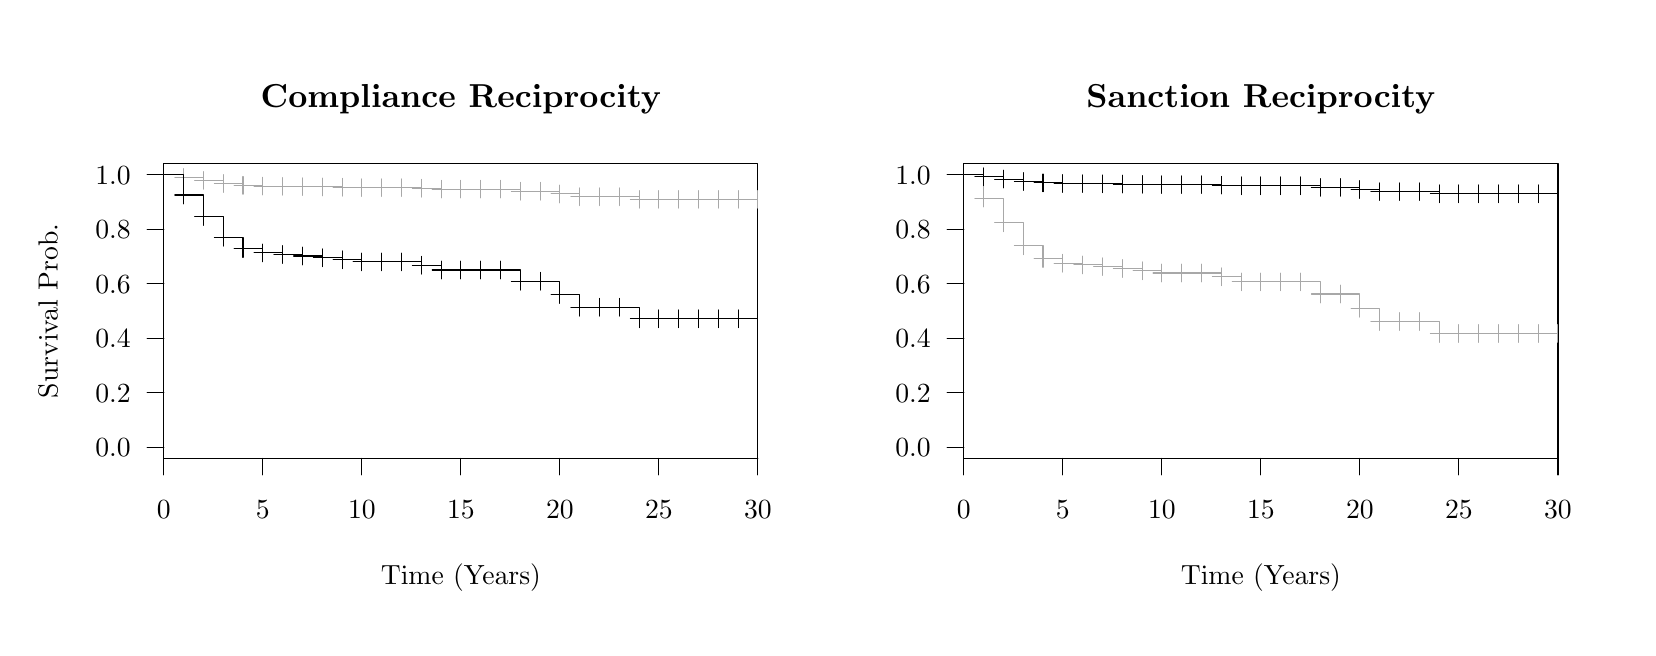
\begin{tikzpicture}[x=1pt,y=1pt]
\definecolor[named]{fillColor}{rgb}{1.00,1.00,1.00}
\path[use as bounding box,fill=fillColor,fill opacity=0.00] (0,0) rectangle (578.16,216.81);
\begin{scope}
\path[clip] (  0.00,  0.00) rectangle (578.16,216.81);
\definecolor[named]{drawColor}{rgb}{0.00,0.00,0.00}

\path[draw=drawColor,line width= 0.4pt,line join=round,line cap=round] ( 49.20, 61.20) -- (263.88, 61.20);

\path[draw=drawColor,line width= 0.4pt,line join=round,line cap=round] ( 49.20, 61.20) -- ( 49.20, 55.20);

\path[draw=drawColor,line width= 0.4pt,line join=round,line cap=round] ( 84.98, 61.20) -- ( 84.98, 55.20);

\path[draw=drawColor,line width= 0.4pt,line join=round,line cap=round] (120.76, 61.20) -- (120.76, 55.20);

\path[draw=drawColor,line width= 0.4pt,line join=round,line cap=round] (156.54, 61.20) -- (156.54, 55.20);

\path[draw=drawColor,line width= 0.4pt,line join=round,line cap=round] (192.32, 61.20) -- (192.32, 55.20);

\path[draw=drawColor,line width= 0.4pt,line join=round,line cap=round] (228.10, 61.20) -- (228.10, 55.20);

\path[draw=drawColor,line width= 0.4pt,line join=round,line cap=round] (263.88, 61.20) -- (263.88, 55.20);

\node[text=drawColor,anchor=base,inner sep=0pt, outer sep=0pt, scale=  1.00] at ( 49.20, 39.60) {0};

\node[text=drawColor,anchor=base,inner sep=0pt, outer sep=0pt, scale=  1.00] at ( 84.98, 39.60) {5};

\node[text=drawColor,anchor=base,inner sep=0pt, outer sep=0pt, scale=  1.00] at (120.76, 39.60) {10};

\node[text=drawColor,anchor=base,inner sep=0pt, outer sep=0pt, scale=  1.00] at (156.54, 39.60) {15};

\node[text=drawColor,anchor=base,inner sep=0pt, outer sep=0pt, scale=  1.00] at (192.32, 39.60) {20};

\node[text=drawColor,anchor=base,inner sep=0pt, outer sep=0pt, scale=  1.00] at (228.10, 39.60) {25};

\node[text=drawColor,anchor=base,inner sep=0pt, outer sep=0pt, scale=  1.00] at (263.88, 39.60) {30};

\path[draw=drawColor,line width= 0.4pt,line join=round,line cap=round] ( 49.20, 65.14) -- ( 49.20,163.67);

\path[draw=drawColor,line width= 0.4pt,line join=round,line cap=round] ( 49.20, 65.14) -- ( 43.20, 65.14);

\path[draw=drawColor,line width= 0.4pt,line join=round,line cap=round] ( 49.20, 84.85) -- ( 43.20, 84.85);

\path[draw=drawColor,line width= 0.4pt,line join=round,line cap=round] ( 49.20,104.55) -- ( 43.20,104.55);

\path[draw=drawColor,line width= 0.4pt,line join=round,line cap=round] ( 49.20,124.26) -- ( 43.20,124.26);

\path[draw=drawColor,line width= 0.4pt,line join=round,line cap=round] ( 49.20,143.96) -- ( 43.20,143.96);

\path[draw=drawColor,line width= 0.4pt,line join=round,line cap=round] ( 49.20,163.67) -- ( 43.20,163.67);

\node[text=drawColor,anchor=base east,inner sep=0pt, outer sep=0pt, scale=  1.00] at ( 37.20, 61.70) {0.0};

\node[text=drawColor,anchor=base east,inner sep=0pt, outer sep=0pt, scale=  1.00] at ( 37.20, 81.40) {0.2};

\node[text=drawColor,anchor=base east,inner sep=0pt, outer sep=0pt, scale=  1.00] at ( 37.20,101.11) {0.4};

\node[text=drawColor,anchor=base east,inner sep=0pt, outer sep=0pt, scale=  1.00] at ( 37.20,120.81) {0.6};

\node[text=drawColor,anchor=base east,inner sep=0pt, outer sep=0pt, scale=  1.00] at ( 37.20,140.52) {0.8};

\node[text=drawColor,anchor=base east,inner sep=0pt, outer sep=0pt, scale=  1.00] at ( 37.20,160.23) {1.0};

\path[draw=drawColor,line width= 0.4pt,line join=round,line cap=round] ( 49.20, 61.20) --
	(263.88, 61.20) --
	(263.88,167.61) --
	( 49.20,167.61) --
	( 49.20, 61.20);
\end{scope}
\begin{scope}
\path[clip] (  0.00,  0.00) rectangle (289.08,216.81);
\definecolor[named]{drawColor}{rgb}{0.00,0.00,0.00}

\node[text=drawColor,anchor=base,inner sep=0pt, outer sep=0pt, scale=  1.20] at (156.54,188.07) {\bfseries Compliance Reciprocity};
\end{scope}
\begin{scope}
\path[clip] ( 49.20, 61.20) rectangle (263.88,167.61);
\definecolor[named]{drawColor}{rgb}{0.66,0.66,0.66}

\path[draw=drawColor,line width= 0.4pt,line join=round,line cap=round] ( 49.20,163.67) --
	( 56.36,163.67) --
	( 56.36,162.71) --
	( 63.51,162.71) --
	( 63.51,161.62) --
	( 70.67,161.62) --
	( 70.67,160.49) --
	( 77.82,160.49) --
	( 77.82,159.82) --
	( 84.98,159.82) --
	( 84.98,159.56) --
	( 92.14,159.56) --
	( 92.14,159.47) --
	( 99.29,159.47) --
	( 99.29,159.37) --
	(106.45,159.37) --
	(106.45,159.26) --
	(113.60,159.26) --
	(113.60,159.13) --
	(120.76,159.13) --
	(120.76,159.00) --
	(142.23,159.00) --
	(142.23,158.78) --
	(149.38,158.78) --
	(149.38,158.47) --
	(178.01,158.47) --
	(178.01,157.71) --
	(192.32,157.71) --
	(192.32,156.73) --
	(199.48,156.73) --
	(199.48,155.74) --
	(220.94,155.74) --
	(220.94,154.76) --
	(464.25,154.76) --
	(464.25,154.76);

\path[draw=drawColor,line width= 0.4pt,line join=round,line cap=round] ( 53.17,162.71) -- ( 59.54,162.71);

\path[draw=drawColor,line width= 0.4pt,line join=round,line cap=round] ( 56.36,159.53) -- ( 56.36,165.90);

\path[draw=drawColor,line width= 0.4pt,line join=round,line cap=round] ( 60.33,161.62) -- ( 66.69,161.62);

\path[draw=drawColor,line width= 0.4pt,line join=round,line cap=round] ( 63.51,158.44) -- ( 63.51,164.80);

\path[draw=drawColor,line width= 0.4pt,line join=round,line cap=round] ( 67.49,160.49) -- ( 73.85,160.49);

\path[draw=drawColor,line width= 0.4pt,line join=round,line cap=round] ( 70.67,157.30) -- ( 70.67,163.67);

\path[draw=drawColor,line width= 0.4pt,line join=round,line cap=round] ( 74.64,159.82) -- ( 81.01,159.82);

\path[draw=drawColor,line width= 0.4pt,line join=round,line cap=round] ( 77.82,156.64) -- ( 77.82,163.01);

\path[draw=drawColor,line width= 0.4pt,line join=round,line cap=round] ( 81.80,159.56) -- ( 88.16,159.56);

\path[draw=drawColor,line width= 0.4pt,line join=round,line cap=round] ( 84.98,156.38) -- ( 84.98,162.74);

\path[draw=drawColor,line width= 0.4pt,line join=round,line cap=round] ( 88.95,159.47) -- ( 95.32,159.47);

\path[draw=drawColor,line width= 0.4pt,line join=round,line cap=round] ( 92.14,156.28) -- ( 92.14,162.65);

\path[draw=drawColor,line width= 0.4pt,line join=round,line cap=round] ( 96.11,159.37) -- (102.47,159.37);

\path[draw=drawColor,line width= 0.4pt,line join=round,line cap=round] ( 99.29,156.19) -- ( 99.29,162.55);

\path[draw=drawColor,line width= 0.4pt,line join=round,line cap=round] (103.27,159.26) -- (109.63,159.26);

\path[draw=drawColor,line width= 0.4pt,line join=round,line cap=round] (106.45,156.08) -- (106.45,162.44);

\path[draw=drawColor,line width= 0.4pt,line join=round,line cap=round] (110.42,159.13) -- (116.79,159.13);

\path[draw=drawColor,line width= 0.4pt,line join=round,line cap=round] (113.60,155.95) -- (113.60,162.31);

\path[draw=drawColor,line width= 0.4pt,line join=round,line cap=round] (117.58,159.00) -- (123.94,159.00);

\path[draw=drawColor,line width= 0.4pt,line join=round,line cap=round] (120.76,155.82) -- (120.76,162.18);

\path[draw=drawColor,line width= 0.4pt,line join=round,line cap=round] (124.73,159.00) -- (131.10,159.00);

\path[draw=drawColor,line width= 0.4pt,line join=round,line cap=round] (127.92,155.82) -- (127.92,162.18);

\path[draw=drawColor,line width= 0.4pt,line join=round,line cap=round] (131.89,159.00) -- (138.25,159.00);

\path[draw=drawColor,line width= 0.4pt,line join=round,line cap=round] (135.07,155.82) -- (135.07,162.18);

\path[draw=drawColor,line width= 0.4pt,line join=round,line cap=round] (139.05,158.78) -- (145.41,158.78);

\path[draw=drawColor,line width= 0.4pt,line join=round,line cap=round] (142.23,155.60) -- (142.23,161.97);

\path[draw=drawColor,line width= 0.4pt,line join=round,line cap=round] (146.20,158.47) -- (152.57,158.47);

\path[draw=drawColor,line width= 0.4pt,line join=round,line cap=round] (149.38,155.29) -- (149.38,161.65);

\path[draw=drawColor,line width= 0.4pt,line join=round,line cap=round] (153.36,158.47) -- (159.72,158.47);

\path[draw=drawColor,line width= 0.4pt,line join=round,line cap=round] (156.54,155.29) -- (156.54,161.65);

\path[draw=drawColor,line width= 0.4pt,line join=round,line cap=round] (160.51,158.47) -- (166.88,158.47);

\path[draw=drawColor,line width= 0.4pt,line join=round,line cap=round] (163.70,155.29) -- (163.70,161.65);

\path[draw=drawColor,line width= 0.4pt,line join=round,line cap=round] (167.67,158.47) -- (174.03,158.47);

\path[draw=drawColor,line width= 0.4pt,line join=round,line cap=round] (170.85,155.29) -- (170.85,161.65);

\path[draw=drawColor,line width= 0.4pt,line join=round,line cap=round] (174.83,157.71) -- (181.19,157.71);

\path[draw=drawColor,line width= 0.4pt,line join=round,line cap=round] (178.01,154.52) -- (178.01,160.89);

\path[draw=drawColor,line width= 0.4pt,line join=round,line cap=round] (181.98,157.71) -- (188.35,157.71);

\path[draw=drawColor,line width= 0.4pt,line join=round,line cap=round] (185.16,154.52) -- (185.16,160.89);

\path[draw=drawColor,line width= 0.4pt,line join=round,line cap=round] (189.14,156.73) -- (195.50,156.73);

\path[draw=drawColor,line width= 0.4pt,line join=round,line cap=round] (192.32,153.55) -- (192.32,159.91);

\path[draw=drawColor,line width= 0.4pt,line join=round,line cap=round] (196.29,155.74) -- (202.66,155.74);

\path[draw=drawColor,line width= 0.4pt,line join=round,line cap=round] (199.48,152.56) -- (199.48,158.92);

\path[draw=drawColor,line width= 0.4pt,line join=round,line cap=round] (203.45,155.74) -- (209.81,155.74);

\path[draw=drawColor,line width= 0.4pt,line join=round,line cap=round] (206.63,152.56) -- (206.63,158.92);

\path[draw=drawColor,line width= 0.4pt,line join=round,line cap=round] (210.61,155.74) -- (216.97,155.74);

\path[draw=drawColor,line width= 0.4pt,line join=round,line cap=round] (213.79,152.56) -- (213.79,158.92);

\path[draw=drawColor,line width= 0.4pt,line join=round,line cap=round] (217.76,154.76) -- (224.13,154.76);

\path[draw=drawColor,line width= 0.4pt,line join=round,line cap=round] (220.94,151.58) -- (220.94,157.95);

\path[draw=drawColor,line width= 0.4pt,line join=round,line cap=round] (224.92,154.76) -- (231.28,154.76);

\path[draw=drawColor,line width= 0.4pt,line join=round,line cap=round] (228.10,151.58) -- (228.10,157.95);

\path[draw=drawColor,line width= 0.4pt,line join=round,line cap=round] (232.07,154.76) -- (238.44,154.76);

\path[draw=drawColor,line width= 0.4pt,line join=round,line cap=round] (235.26,151.58) -- (235.26,157.95);

\path[draw=drawColor,line width= 0.4pt,line join=round,line cap=round] (239.23,154.76) -- (245.59,154.76);

\path[draw=drawColor,line width= 0.4pt,line join=round,line cap=round] (242.41,151.58) -- (242.41,157.95);

\path[draw=drawColor,line width= 0.4pt,line join=round,line cap=round] (246.39,154.76) -- (252.75,154.76);

\path[draw=drawColor,line width= 0.4pt,line join=round,line cap=round] (249.57,151.58) -- (249.57,157.95);

\path[draw=drawColor,line width= 0.4pt,line join=round,line cap=round] (253.54,154.76) -- (259.91,154.76);

\path[draw=drawColor,line width= 0.4pt,line join=round,line cap=round] (256.72,151.58) -- (256.72,157.95);

\path[draw=drawColor,line width= 0.4pt,line join=round,line cap=round] (260.70,154.76) -- (267.06,154.76);

\path[draw=drawColor,line width= 0.4pt,line join=round,line cap=round] (263.88,151.58) -- (263.88,157.95);

\path[draw=drawColor,line width= 0.4pt,line join=round,line cap=round] (267.85,154.76) -- (274.22,154.76);

\path[draw=drawColor,line width= 0.4pt,line join=round,line cap=round] (271.04,151.58) -- (271.04,157.95);

\path[draw=drawColor,line width= 0.4pt,line join=round,line cap=round] (275.01,154.76) -- (281.37,154.76);

\path[draw=drawColor,line width= 0.4pt,line join=round,line cap=round] (278.19,151.58) -- (278.19,157.95);

\path[draw=drawColor,line width= 0.4pt,line join=round,line cap=round] (282.17,154.76) -- (288.53,154.76);

\path[draw=drawColor,line width= 0.4pt,line join=round,line cap=round] (285.35,151.58) -- (285.35,157.95);

\path[draw=drawColor,line width= 0.4pt,line join=round,line cap=round] (289.32,154.76) -- (295.69,154.76);

\path[draw=drawColor,line width= 0.4pt,line join=round,line cap=round] (292.50,151.58) -- (292.50,157.95);

\path[draw=drawColor,line width= 0.4pt,line join=round,line cap=round] (296.48,154.76) -- (302.84,154.76);

\path[draw=drawColor,line width= 0.4pt,line join=round,line cap=round] (299.66,151.58) -- (299.66,157.95);

\path[draw=drawColor,line width= 0.4pt,line join=round,line cap=round] (303.63,154.76) -- (310.00,154.76);

\path[draw=drawColor,line width= 0.4pt,line join=round,line cap=round] (306.82,151.58) -- (306.82,157.95);

\path[draw=drawColor,line width= 0.4pt,line join=round,line cap=round] (310.79,154.76) -- (317.15,154.76);

\path[draw=drawColor,line width= 0.4pt,line join=round,line cap=round] (313.97,151.58) -- (313.97,157.95);

\path[draw=drawColor,line width= 0.4pt,line join=round,line cap=round] (317.95,154.76) -- (324.31,154.76);

\path[draw=drawColor,line width= 0.4pt,line join=round,line cap=round] (321.13,151.58) -- (321.13,157.95);

\path[draw=drawColor,line width= 0.4pt,line join=round,line cap=round] (325.10,154.76) -- (331.47,154.76);

\path[draw=drawColor,line width= 0.4pt,line join=round,line cap=round] (328.28,151.58) -- (328.28,157.95);

\path[draw=drawColor,line width= 0.4pt,line join=round,line cap=round] (332.26,154.76) -- (338.62,154.76);

\path[draw=drawColor,line width= 0.4pt,line join=round,line cap=round] (335.44,151.58) -- (335.44,157.95);

\path[draw=drawColor,line width= 0.4pt,line join=round,line cap=round] (339.41,154.76) -- (345.78,154.76);

\path[draw=drawColor,line width= 0.4pt,line join=round,line cap=round] (342.60,151.58) -- (342.60,157.95);

\path[draw=drawColor,line width= 0.4pt,line join=round,line cap=round] (346.57,154.76) -- (352.93,154.76);

\path[draw=drawColor,line width= 0.4pt,line join=round,line cap=round] (349.75,151.58) -- (349.75,157.95);

\path[draw=drawColor,line width= 0.4pt,line join=round,line cap=round] (353.73,154.76) -- (360.09,154.76);

\path[draw=drawColor,line width= 0.4pt,line join=round,line cap=round] (356.91,151.58) -- (356.91,157.95);

\path[draw=drawColor,line width= 0.4pt,line join=round,line cap=round] (360.88,154.76) -- (367.25,154.76);

\path[draw=drawColor,line width= 0.4pt,line join=round,line cap=round] (364.06,151.58) -- (364.06,157.95);

\path[draw=drawColor,line width= 0.4pt,line join=round,line cap=round] (368.04,154.76) -- (374.40,154.76);

\path[draw=drawColor,line width= 0.4pt,line join=round,line cap=round] (371.22,151.58) -- (371.22,157.95);

\path[draw=drawColor,line width= 0.4pt,line join=round,line cap=round] (375.19,154.76) -- (381.56,154.76);

\path[draw=drawColor,line width= 0.4pt,line join=round,line cap=round] (378.38,151.58) -- (378.38,157.95);

\path[draw=drawColor,line width= 0.4pt,line join=round,line cap=round] (382.35,154.76) -- (388.71,154.76);

\path[draw=drawColor,line width= 0.4pt,line join=round,line cap=round] (385.53,151.58) -- (385.53,157.95);

\path[draw=drawColor,line width= 0.4pt,line join=round,line cap=round] (389.51,154.76) -- (395.87,154.76);

\path[draw=drawColor,line width= 0.4pt,line join=round,line cap=round] (392.69,151.58) -- (392.69,157.95);

\path[draw=drawColor,line width= 0.4pt,line join=round,line cap=round] (396.66,154.76) -- (403.03,154.76);

\path[draw=drawColor,line width= 0.4pt,line join=round,line cap=round] (399.84,151.58) -- (399.84,157.95);

\path[draw=drawColor,line width= 0.4pt,line join=round,line cap=round] (403.82,154.76) -- (410.18,154.76);

\path[draw=drawColor,line width= 0.4pt,line join=round,line cap=round] (407.00,151.58) -- (407.00,157.95);

\path[draw=drawColor,line width= 0.4pt,line join=round,line cap=round] (410.97,154.76) -- (417.34,154.76);

\path[draw=drawColor,line width= 0.4pt,line join=round,line cap=round] (414.16,151.58) -- (414.16,157.95);

\path[draw=drawColor,line width= 0.4pt,line join=round,line cap=round] (418.13,154.76) -- (424.49,154.76);

\path[draw=drawColor,line width= 0.4pt,line join=round,line cap=round] (421.31,151.58) -- (421.31,157.95);

\path[draw=drawColor,line width= 0.4pt,line join=round,line cap=round] (425.29,154.76) -- (431.65,154.76);

\path[draw=drawColor,line width= 0.4pt,line join=round,line cap=round] (428.47,151.58) -- (428.47,157.95);

\path[draw=drawColor,line width= 0.4pt,line join=round,line cap=round] (432.44,154.76) -- (438.81,154.76);

\path[draw=drawColor,line width= 0.4pt,line join=round,line cap=round] (435.62,151.58) -- (435.62,157.95);

\path[draw=drawColor,line width= 0.4pt,line join=round,line cap=round] (439.60,154.76) -- (445.96,154.76);

\path[draw=drawColor,line width= 0.4pt,line join=round,line cap=round] (442.78,151.58) -- (442.78,157.95);

\path[draw=drawColor,line width= 0.4pt,line join=round,line cap=round] (446.75,154.76) -- (453.12,154.76);

\path[draw=drawColor,line width= 0.4pt,line join=round,line cap=round] (449.94,151.58) -- (449.94,157.95);

\path[draw=drawColor,line width= 0.4pt,line join=round,line cap=round] (453.91,154.76) -- (460.27,154.76);

\path[draw=drawColor,line width= 0.4pt,line join=round,line cap=round] (457.09,151.58) -- (457.09,157.95);

\path[draw=drawColor,line width= 0.4pt,line join=round,line cap=round] (461.07,154.76) -- (467.43,154.76);

\path[draw=drawColor,line width= 0.4pt,line join=round,line cap=round] (464.25,151.58) -- (464.25,157.95);
\definecolor[named]{drawColor}{rgb}{0.00,0.00,0.00}

\path[draw=drawColor,line width= 0.4pt,line join=round,line cap=round] ( 49.20,163.67) --
	( 56.36,163.67) --
	( 56.36,156.34) --
	( 63.51,156.34) --
	( 63.51,148.53) --
	( 70.67,148.53) --
	( 70.67,141.08) --
	( 77.82,141.08) --
	( 77.82,136.99) --
	( 84.98,136.99) --
	( 84.98,135.42) --
	( 92.14,135.42) --
	( 92.14,134.87) --
	( 99.29,134.87) --
	( 99.29,134.31) --
	(106.45,134.31) --
	(106.45,133.67) --
	(113.60,133.67) --
	(113.60,132.94) --
	(120.76,132.94) --
	(120.76,132.18) --
	(142.23,132.18) --
	(142.23,130.97) --
	(149.38,130.97) --
	(149.38,129.25) --
	(178.01,129.25) --
	(178.01,125.19) --
	(192.32,125.19) --
	(192.32,120.36) --
	(199.48,120.36) --
	(199.48,115.80) --
	(220.94,115.80) --
	(220.94,111.63) --
	(464.25,111.63) --
	(464.25,111.63);

\path[draw=drawColor,line width= 0.4pt,line join=round,line cap=round] ( 53.17,156.34) -- ( 59.54,156.34);

\path[draw=drawColor,line width= 0.4pt,line join=round,line cap=round] ( 56.36,153.16) -- ( 56.36,159.52);

\path[draw=drawColor,line width= 0.4pt,line join=round,line cap=round] ( 60.33,148.53) -- ( 66.69,148.53);

\path[draw=drawColor,line width= 0.4pt,line join=round,line cap=round] ( 63.51,145.35) -- ( 63.51,151.71);

\path[draw=drawColor,line width= 0.4pt,line join=round,line cap=round] ( 67.49,141.08) -- ( 73.85,141.08);

\path[draw=drawColor,line width= 0.4pt,line join=round,line cap=round] ( 70.67,137.90) -- ( 70.67,144.26);

\path[draw=drawColor,line width= 0.4pt,line join=round,line cap=round] ( 74.64,136.99) -- ( 81.01,136.99);

\path[draw=drawColor,line width= 0.4pt,line join=round,line cap=round] ( 77.82,133.81) -- ( 77.82,140.17);

\path[draw=drawColor,line width= 0.4pt,line join=round,line cap=round] ( 81.80,135.42) -- ( 88.16,135.42);

\path[draw=drawColor,line width= 0.4pt,line join=round,line cap=round] ( 84.98,132.24) -- ( 84.98,138.60);

\path[draw=drawColor,line width= 0.4pt,line join=round,line cap=round] ( 88.95,134.87) -- ( 95.32,134.87);

\path[draw=drawColor,line width= 0.4pt,line join=round,line cap=round] ( 92.14,131.68) -- ( 92.14,138.05);

\path[draw=drawColor,line width= 0.4pt,line join=round,line cap=round] ( 96.11,134.31) -- (102.47,134.31);

\path[draw=drawColor,line width= 0.4pt,line join=round,line cap=round] ( 99.29,131.13) -- ( 99.29,137.49);

\path[draw=drawColor,line width= 0.4pt,line join=round,line cap=round] (103.27,133.67) -- (109.63,133.67);

\path[draw=drawColor,line width= 0.4pt,line join=round,line cap=round] (106.45,130.49) -- (106.45,136.85);

\path[draw=drawColor,line width= 0.4pt,line join=round,line cap=round] (110.42,132.94) -- (116.79,132.94);

\path[draw=drawColor,line width= 0.4pt,line join=round,line cap=round] (113.60,129.75) -- (113.60,136.12);

\path[draw=drawColor,line width= 0.4pt,line join=round,line cap=round] (117.58,132.18) -- (123.94,132.18);

\path[draw=drawColor,line width= 0.4pt,line join=round,line cap=round] (120.76,128.99) -- (120.76,135.36);

\path[draw=drawColor,line width= 0.4pt,line join=round,line cap=round] (124.73,132.18) -- (131.10,132.18);

\path[draw=drawColor,line width= 0.4pt,line join=round,line cap=round] (127.92,128.99) -- (127.92,135.36);

\path[draw=drawColor,line width= 0.4pt,line join=round,line cap=round] (131.89,132.18) -- (138.25,132.18);

\path[draw=drawColor,line width= 0.4pt,line join=round,line cap=round] (135.07,128.99) -- (135.07,135.36);

\path[draw=drawColor,line width= 0.4pt,line join=round,line cap=round] (139.05,130.97) -- (145.41,130.97);

\path[draw=drawColor,line width= 0.4pt,line join=round,line cap=round] (142.23,127.79) -- (142.23,134.15);

\path[draw=drawColor,line width= 0.4pt,line join=round,line cap=round] (146.20,129.25) -- (152.57,129.25);

\path[draw=drawColor,line width= 0.4pt,line join=round,line cap=round] (149.38,126.06) -- (149.38,132.43);

\path[draw=drawColor,line width= 0.4pt,line join=round,line cap=round] (153.36,129.25) -- (159.72,129.25);

\path[draw=drawColor,line width= 0.4pt,line join=round,line cap=round] (156.54,126.06) -- (156.54,132.43);

\path[draw=drawColor,line width= 0.4pt,line join=round,line cap=round] (160.51,129.25) -- (166.88,129.25);

\path[draw=drawColor,line width= 0.4pt,line join=round,line cap=round] (163.70,126.06) -- (163.70,132.43);

\path[draw=drawColor,line width= 0.4pt,line join=round,line cap=round] (167.67,129.25) -- (174.03,129.25);

\path[draw=drawColor,line width= 0.4pt,line join=round,line cap=round] (170.85,126.06) -- (170.85,132.43);

\path[draw=drawColor,line width= 0.4pt,line join=round,line cap=round] (174.83,125.19) -- (181.19,125.19);

\path[draw=drawColor,line width= 0.4pt,line join=round,line cap=round] (178.01,122.01) -- (178.01,128.38);

\path[draw=drawColor,line width= 0.4pt,line join=round,line cap=round] (181.98,125.19) -- (188.35,125.19);

\path[draw=drawColor,line width= 0.4pt,line join=round,line cap=round] (185.16,122.01) -- (185.16,128.38);

\path[draw=drawColor,line width= 0.4pt,line join=round,line cap=round] (189.14,120.36) -- (195.50,120.36);

\path[draw=drawColor,line width= 0.4pt,line join=round,line cap=round] (192.32,117.18) -- (192.32,123.54);

\path[draw=drawColor,line width= 0.4pt,line join=round,line cap=round] (196.29,115.80) -- (202.66,115.80);

\path[draw=drawColor,line width= 0.4pt,line join=round,line cap=round] (199.48,112.62) -- (199.48,118.99);

\path[draw=drawColor,line width= 0.4pt,line join=round,line cap=round] (203.45,115.80) -- (209.81,115.80);

\path[draw=drawColor,line width= 0.4pt,line join=round,line cap=round] (206.63,112.62) -- (206.63,118.99);

\path[draw=drawColor,line width= 0.4pt,line join=round,line cap=round] (210.61,115.80) -- (216.97,115.80);

\path[draw=drawColor,line width= 0.4pt,line join=round,line cap=round] (213.79,112.62) -- (213.79,118.99);

\path[draw=drawColor,line width= 0.4pt,line join=round,line cap=round] (217.76,111.63) -- (224.13,111.63);

\path[draw=drawColor,line width= 0.4pt,line join=round,line cap=round] (220.94,108.44) -- (220.94,114.81);

\path[draw=drawColor,line width= 0.4pt,line join=round,line cap=round] (224.92,111.63) -- (231.28,111.63);

\path[draw=drawColor,line width= 0.4pt,line join=round,line cap=round] (228.10,108.44) -- (228.10,114.81);

\path[draw=drawColor,line width= 0.4pt,line join=round,line cap=round] (232.07,111.63) -- (238.44,111.63);

\path[draw=drawColor,line width= 0.4pt,line join=round,line cap=round] (235.26,108.44) -- (235.26,114.81);

\path[draw=drawColor,line width= 0.4pt,line join=round,line cap=round] (239.23,111.63) -- (245.59,111.63);

\path[draw=drawColor,line width= 0.4pt,line join=round,line cap=round] (242.41,108.44) -- (242.41,114.81);

\path[draw=drawColor,line width= 0.4pt,line join=round,line cap=round] (246.39,111.63) -- (252.75,111.63);

\path[draw=drawColor,line width= 0.4pt,line join=round,line cap=round] (249.57,108.44) -- (249.57,114.81);

\path[draw=drawColor,line width= 0.4pt,line join=round,line cap=round] (253.54,111.63) -- (259.91,111.63);

\path[draw=drawColor,line width= 0.4pt,line join=round,line cap=round] (256.72,108.44) -- (256.72,114.81);

\path[draw=drawColor,line width= 0.4pt,line join=round,line cap=round] (260.70,111.63) -- (267.06,111.63);

\path[draw=drawColor,line width= 0.4pt,line join=round,line cap=round] (263.88,108.44) -- (263.88,114.81);

\path[draw=drawColor,line width= 0.4pt,line join=round,line cap=round] (267.85,111.63) -- (274.22,111.63);

\path[draw=drawColor,line width= 0.4pt,line join=round,line cap=round] (271.04,108.44) -- (271.04,114.81);

\path[draw=drawColor,line width= 0.4pt,line join=round,line cap=round] (275.01,111.63) -- (281.37,111.63);

\path[draw=drawColor,line width= 0.4pt,line join=round,line cap=round] (278.19,108.44) -- (278.19,114.81);

\path[draw=drawColor,line width= 0.4pt,line join=round,line cap=round] (282.17,111.63) -- (288.53,111.63);

\path[draw=drawColor,line width= 0.4pt,line join=round,line cap=round] (285.35,108.44) -- (285.35,114.81);

\path[draw=drawColor,line width= 0.4pt,line join=round,line cap=round] (289.32,111.63) -- (295.69,111.63);

\path[draw=drawColor,line width= 0.4pt,line join=round,line cap=round] (292.50,108.44) -- (292.50,114.81);

\path[draw=drawColor,line width= 0.4pt,line join=round,line cap=round] (296.48,111.63) -- (302.84,111.63);

\path[draw=drawColor,line width= 0.4pt,line join=round,line cap=round] (299.66,108.44) -- (299.66,114.81);

\path[draw=drawColor,line width= 0.4pt,line join=round,line cap=round] (303.63,111.63) -- (310.00,111.63);

\path[draw=drawColor,line width= 0.4pt,line join=round,line cap=round] (306.82,108.44) -- (306.82,114.81);

\path[draw=drawColor,line width= 0.4pt,line join=round,line cap=round] (310.79,111.63) -- (317.15,111.63);

\path[draw=drawColor,line width= 0.4pt,line join=round,line cap=round] (313.97,108.44) -- (313.97,114.81);

\path[draw=drawColor,line width= 0.4pt,line join=round,line cap=round] (317.95,111.63) -- (324.31,111.63);

\path[draw=drawColor,line width= 0.4pt,line join=round,line cap=round] (321.13,108.44) -- (321.13,114.81);

\path[draw=drawColor,line width= 0.4pt,line join=round,line cap=round] (325.10,111.63) -- (331.47,111.63);

\path[draw=drawColor,line width= 0.4pt,line join=round,line cap=round] (328.28,108.44) -- (328.28,114.81);

\path[draw=drawColor,line width= 0.4pt,line join=round,line cap=round] (332.26,111.63) -- (338.62,111.63);

\path[draw=drawColor,line width= 0.4pt,line join=round,line cap=round] (335.44,108.44) -- (335.44,114.81);

\path[draw=drawColor,line width= 0.4pt,line join=round,line cap=round] (339.41,111.63) -- (345.78,111.63);

\path[draw=drawColor,line width= 0.4pt,line join=round,line cap=round] (342.60,108.44) -- (342.60,114.81);

\path[draw=drawColor,line width= 0.4pt,line join=round,line cap=round] (346.57,111.63) -- (352.93,111.63);

\path[draw=drawColor,line width= 0.4pt,line join=round,line cap=round] (349.75,108.44) -- (349.75,114.81);

\path[draw=drawColor,line width= 0.4pt,line join=round,line cap=round] (353.73,111.63) -- (360.09,111.63);

\path[draw=drawColor,line width= 0.4pt,line join=round,line cap=round] (356.91,108.44) -- (356.91,114.81);

\path[draw=drawColor,line width= 0.4pt,line join=round,line cap=round] (360.88,111.63) -- (367.25,111.63);

\path[draw=drawColor,line width= 0.4pt,line join=round,line cap=round] (364.06,108.44) -- (364.06,114.81);

\path[draw=drawColor,line width= 0.4pt,line join=round,line cap=round] (368.04,111.63) -- (374.40,111.63);

\path[draw=drawColor,line width= 0.4pt,line join=round,line cap=round] (371.22,108.44) -- (371.22,114.81);

\path[draw=drawColor,line width= 0.4pt,line join=round,line cap=round] (375.19,111.63) -- (381.56,111.63);

\path[draw=drawColor,line width= 0.4pt,line join=round,line cap=round] (378.38,108.44) -- (378.38,114.81);

\path[draw=drawColor,line width= 0.4pt,line join=round,line cap=round] (382.35,111.63) -- (388.71,111.63);

\path[draw=drawColor,line width= 0.4pt,line join=round,line cap=round] (385.53,108.44) -- (385.53,114.81);

\path[draw=drawColor,line width= 0.4pt,line join=round,line cap=round] (389.51,111.63) -- (395.87,111.63);

\path[draw=drawColor,line width= 0.4pt,line join=round,line cap=round] (392.69,108.44) -- (392.69,114.81);

\path[draw=drawColor,line width= 0.4pt,line join=round,line cap=round] (396.66,111.63) -- (403.03,111.63);

\path[draw=drawColor,line width= 0.4pt,line join=round,line cap=round] (399.84,108.44) -- (399.84,114.81);

\path[draw=drawColor,line width= 0.4pt,line join=round,line cap=round] (403.82,111.63) -- (410.18,111.63);

\path[draw=drawColor,line width= 0.4pt,line join=round,line cap=round] (407.00,108.44) -- (407.00,114.81);

\path[draw=drawColor,line width= 0.4pt,line join=round,line cap=round] (410.97,111.63) -- (417.34,111.63);

\path[draw=drawColor,line width= 0.4pt,line join=round,line cap=round] (414.16,108.44) -- (414.16,114.81);

\path[draw=drawColor,line width= 0.4pt,line join=round,line cap=round] (418.13,111.63) -- (424.49,111.63);

\path[draw=drawColor,line width= 0.4pt,line join=round,line cap=round] (421.31,108.44) -- (421.31,114.81);

\path[draw=drawColor,line width= 0.4pt,line join=round,line cap=round] (425.29,111.63) -- (431.65,111.63);

\path[draw=drawColor,line width= 0.4pt,line join=round,line cap=round] (428.47,108.44) -- (428.47,114.81);

\path[draw=drawColor,line width= 0.4pt,line join=round,line cap=round] (432.44,111.63) -- (438.81,111.63);

\path[draw=drawColor,line width= 0.4pt,line join=round,line cap=round] (435.62,108.44) -- (435.62,114.81);

\path[draw=drawColor,line width= 0.4pt,line join=round,line cap=round] (439.60,111.63) -- (445.96,111.63);

\path[draw=drawColor,line width= 0.4pt,line join=round,line cap=round] (442.78,108.44) -- (442.78,114.81);

\path[draw=drawColor,line width= 0.4pt,line join=round,line cap=round] (446.75,111.63) -- (453.12,111.63);

\path[draw=drawColor,line width= 0.4pt,line join=round,line cap=round] (449.94,108.44) -- (449.94,114.81);

\path[draw=drawColor,line width= 0.4pt,line join=round,line cap=round] (453.91,111.63) -- (460.27,111.63);

\path[draw=drawColor,line width= 0.4pt,line join=round,line cap=round] (457.09,108.44) -- (457.09,114.81);

\path[draw=drawColor,line width= 0.4pt,line join=round,line cap=round] (461.07,111.63) -- (467.43,111.63);

\path[draw=drawColor,line width= 0.4pt,line join=round,line cap=round] (464.25,108.44) -- (464.25,114.81);
\end{scope}
\begin{scope}
\path[clip] (  0.00,  0.00) rectangle (289.08,216.81);
\definecolor[named]{drawColor}{rgb}{0.00,0.00,0.00}

\node[text=drawColor,rotate= 90.00,anchor=base,inner sep=0pt, outer sep=0pt, scale=  1.00] at ( 10.80,114.41) {Survival Prob.};

\node[text=drawColor,anchor=base,inner sep=0pt, outer sep=0pt, scale=  1.00] at (156.54, 15.60) {Time (Years)};
\end{scope}
\begin{scope}
\path[clip] (  0.00,  0.00) rectangle (578.16,216.81);
\definecolor[named]{drawColor}{rgb}{0.00,0.00,0.00}

\path[draw=drawColor,line width= 0.4pt,line join=round,line cap=round] (338.28, 61.20) -- (552.96, 61.20);

\path[draw=drawColor,line width= 0.4pt,line join=round,line cap=round] (338.28, 61.20) -- (338.28, 55.20);

\path[draw=drawColor,line width= 0.4pt,line join=round,line cap=round] (374.06, 61.20) -- (374.06, 55.20);

\path[draw=drawColor,line width= 0.4pt,line join=round,line cap=round] (409.84, 61.20) -- (409.84, 55.20);

\path[draw=drawColor,line width= 0.4pt,line join=round,line cap=round] (445.62, 61.20) -- (445.62, 55.20);

\path[draw=drawColor,line width= 0.4pt,line join=round,line cap=round] (481.40, 61.20) -- (481.40, 55.20);

\path[draw=drawColor,line width= 0.4pt,line join=round,line cap=round] (517.18, 61.20) -- (517.18, 55.20);

\path[draw=drawColor,line width= 0.4pt,line join=round,line cap=round] (552.96, 61.20) -- (552.96, 55.20);

\node[text=drawColor,anchor=base,inner sep=0pt, outer sep=0pt, scale=  1.00] at (338.28, 39.60) {0};

\node[text=drawColor,anchor=base,inner sep=0pt, outer sep=0pt, scale=  1.00] at (374.06, 39.60) {5};

\node[text=drawColor,anchor=base,inner sep=0pt, outer sep=0pt, scale=  1.00] at (409.84, 39.60) {10};

\node[text=drawColor,anchor=base,inner sep=0pt, outer sep=0pt, scale=  1.00] at (445.62, 39.60) {15};

\node[text=drawColor,anchor=base,inner sep=0pt, outer sep=0pt, scale=  1.00] at (481.40, 39.60) {20};

\node[text=drawColor,anchor=base,inner sep=0pt, outer sep=0pt, scale=  1.00] at (517.18, 39.60) {25};

\node[text=drawColor,anchor=base,inner sep=0pt, outer sep=0pt, scale=  1.00] at (552.96, 39.60) {30};

\path[draw=drawColor,line width= 0.4pt,line join=round,line cap=round] (338.28, 65.14) -- (338.28,163.67);

\path[draw=drawColor,line width= 0.4pt,line join=round,line cap=round] (338.28, 65.14) -- (332.28, 65.14);

\path[draw=drawColor,line width= 0.4pt,line join=round,line cap=round] (338.28, 84.85) -- (332.28, 84.85);

\path[draw=drawColor,line width= 0.4pt,line join=round,line cap=round] (338.28,104.55) -- (332.28,104.55);

\path[draw=drawColor,line width= 0.4pt,line join=round,line cap=round] (338.28,124.26) -- (332.28,124.26);

\path[draw=drawColor,line width= 0.4pt,line join=round,line cap=round] (338.28,143.96) -- (332.28,143.96);

\path[draw=drawColor,line width= 0.4pt,line join=round,line cap=round] (338.28,163.67) -- (332.28,163.67);

\node[text=drawColor,anchor=base east,inner sep=0pt, outer sep=0pt, scale=  1.00] at (326.28, 61.70) {0.0};

\node[text=drawColor,anchor=base east,inner sep=0pt, outer sep=0pt, scale=  1.00] at (326.28, 81.40) {0.2};

\node[text=drawColor,anchor=base east,inner sep=0pt, outer sep=0pt, scale=  1.00] at (326.28,101.11) {0.4};

\node[text=drawColor,anchor=base east,inner sep=0pt, outer sep=0pt, scale=  1.00] at (326.28,120.81) {0.6};

\node[text=drawColor,anchor=base east,inner sep=0pt, outer sep=0pt, scale=  1.00] at (326.28,140.52) {0.8};

\node[text=drawColor,anchor=base east,inner sep=0pt, outer sep=0pt, scale=  1.00] at (326.28,160.23) {1.0};

\path[draw=drawColor,line width= 0.4pt,line join=round,line cap=round] (338.28, 61.20) --
	(552.96, 61.20) --
	(552.96,167.61) --
	(338.28,167.61) --
	(338.28, 61.20);
\end{scope}
\begin{scope}
\path[clip] (289.08,  0.00) rectangle (578.16,216.81);
\definecolor[named]{drawColor}{rgb}{0.00,0.00,0.00}

\node[text=drawColor,anchor=base,inner sep=0pt, outer sep=0pt, scale=  1.20] at (445.62,188.07) {\bfseries Sanction Reciprocity};
\end{scope}
\begin{scope}
\path[clip] (338.28, 61.20) rectangle (552.96,167.61);
\definecolor[named]{drawColor}{rgb}{0.66,0.66,0.66}

\path[draw=drawColor,line width= 0.4pt,line join=round,line cap=round] (338.28,163.67) --
	(345.44,163.67) --
	(345.44,155.21) --
	(352.59,155.21) --
	(352.59,146.32) --
	(359.75,146.32) --
	(359.75,137.96) --
	(366.90,137.96) --
	(366.90,133.42) --
	(374.06,133.42) --
	(374.06,131.69) --
	(381.22,131.69) --
	(381.22,131.08) --
	(388.37,131.08) --
	(388.37,130.47) --
	(395.53,130.47) --
	(395.53,129.77) --
	(402.68,129.77) --
	(402.68,128.97) --
	(409.84,128.97) --
	(409.84,128.14) --
	(431.31,128.14) --
	(431.31,126.82) --
	(438.46,126.82) --
	(438.46,124.95) --
	(467.09,124.95) --
	(467.09,120.58) --
	(481.40,120.58) --
	(481.40,115.43) --
	(488.56,115.43) --
	(488.56,110.65) --
	(510.02,110.65) --
	(510.02,106.32) --
	(578.16,106.32);

\path[draw=drawColor,line width= 0.4pt,line join=round,line cap=round] (342.25,155.21) -- (348.62,155.21);

\path[draw=drawColor,line width= 0.4pt,line join=round,line cap=round] (345.44,152.03) -- (345.44,158.39);

\path[draw=drawColor,line width= 0.4pt,line join=round,line cap=round] (349.41,146.32) -- (355.77,146.32);

\path[draw=drawColor,line width= 0.4pt,line join=round,line cap=round] (352.59,143.14) -- (352.59,149.50);

\path[draw=drawColor,line width= 0.4pt,line join=round,line cap=round] (356.57,137.96) -- (362.93,137.96);

\path[draw=drawColor,line width= 0.4pt,line join=round,line cap=round] (359.75,134.78) -- (359.75,141.14);

\path[draw=drawColor,line width= 0.4pt,line join=round,line cap=round] (363.72,133.42) -- (370.09,133.42);

\path[draw=drawColor,line width= 0.4pt,line join=round,line cap=round] (366.90,130.24) -- (366.90,136.61);

\path[draw=drawColor,line width= 0.4pt,line join=round,line cap=round] (370.88,131.69) -- (377.24,131.69);

\path[draw=drawColor,line width= 0.4pt,line join=round,line cap=round] (374.06,128.51) -- (374.06,134.88);

\path[draw=drawColor,line width= 0.4pt,line join=round,line cap=round] (378.03,131.08) -- (384.40,131.08);

\path[draw=drawColor,line width= 0.4pt,line join=round,line cap=round] (381.22,127.90) -- (381.22,134.26);

\path[draw=drawColor,line width= 0.4pt,line join=round,line cap=round] (385.19,130.47) -- (391.55,130.47);

\path[draw=drawColor,line width= 0.4pt,line join=round,line cap=round] (388.37,127.29) -- (388.37,133.65);

\path[draw=drawColor,line width= 0.4pt,line join=round,line cap=round] (392.35,129.77) -- (398.71,129.77);

\path[draw=drawColor,line width= 0.4pt,line join=round,line cap=round] (395.53,126.59) -- (395.53,132.95);

\path[draw=drawColor,line width= 0.4pt,line join=round,line cap=round] (399.50,128.97) -- (405.87,128.97);

\path[draw=drawColor,line width= 0.4pt,line join=round,line cap=round] (402.68,125.78) -- (402.68,132.15);

\path[draw=drawColor,line width= 0.4pt,line join=round,line cap=round] (406.66,128.14) -- (413.02,128.14);

\path[draw=drawColor,line width= 0.4pt,line join=round,line cap=round] (409.84,124.96) -- (409.84,131.32);

\path[draw=drawColor,line width= 0.4pt,line join=round,line cap=round] (413.81,128.14) -- (420.18,128.14);

\path[draw=drawColor,line width= 0.4pt,line join=round,line cap=round] (417.00,124.96) -- (417.00,131.32);

\path[draw=drawColor,line width= 0.4pt,line join=round,line cap=round] (420.97,128.14) -- (427.33,128.14);

\path[draw=drawColor,line width= 0.4pt,line join=round,line cap=round] (424.15,124.96) -- (424.15,131.32);

\path[draw=drawColor,line width= 0.4pt,line join=round,line cap=round] (428.13,126.82) -- (434.49,126.82);

\path[draw=drawColor,line width= 0.4pt,line join=round,line cap=round] (431.31,123.64) -- (431.31,130.01);

\path[draw=drawColor,line width= 0.4pt,line join=round,line cap=round] (435.28,124.95) -- (441.65,124.95);

\path[draw=drawColor,line width= 0.4pt,line join=round,line cap=round] (438.46,121.77) -- (438.46,128.13);

\path[draw=drawColor,line width= 0.4pt,line join=round,line cap=round] (442.44,124.95) -- (448.80,124.95);

\path[draw=drawColor,line width= 0.4pt,line join=round,line cap=round] (445.62,121.77) -- (445.62,128.13);

\path[draw=drawColor,line width= 0.4pt,line join=round,line cap=round] (449.59,124.95) -- (455.96,124.95);

\path[draw=drawColor,line width= 0.4pt,line join=round,line cap=round] (452.78,121.77) -- (452.78,128.13);

\path[draw=drawColor,line width= 0.4pt,line join=round,line cap=round] (456.75,124.95) -- (463.11,124.95);

\path[draw=drawColor,line width= 0.4pt,line join=round,line cap=round] (459.93,121.77) -- (459.93,128.13);

\path[draw=drawColor,line width= 0.4pt,line join=round,line cap=round] (463.91,120.58) -- (470.27,120.58);

\path[draw=drawColor,line width= 0.4pt,line join=round,line cap=round] (467.09,117.40) -- (467.09,123.77);

\path[draw=drawColor,line width= 0.4pt,line join=round,line cap=round] (471.06,120.58) -- (477.43,120.58);

\path[draw=drawColor,line width= 0.4pt,line join=round,line cap=round] (474.24,117.40) -- (474.24,123.77);

\path[draw=drawColor,line width= 0.4pt,line join=round,line cap=round] (478.22,115.43) -- (484.58,115.43);

\path[draw=drawColor,line width= 0.4pt,line join=round,line cap=round] (481.40,112.25) -- (481.40,118.62);

\path[draw=drawColor,line width= 0.4pt,line join=round,line cap=round] (485.37,110.65) -- (491.74,110.65);

\path[draw=drawColor,line width= 0.4pt,line join=round,line cap=round] (488.56,107.47) -- (488.56,113.83);

\path[draw=drawColor,line width= 0.4pt,line join=round,line cap=round] (492.53,110.65) -- (498.89,110.65);

\path[draw=drawColor,line width= 0.4pt,line join=round,line cap=round] (495.71,107.47) -- (495.71,113.83);

\path[draw=drawColor,line width= 0.4pt,line join=round,line cap=round] (499.69,110.65) -- (506.05,110.65);

\path[draw=drawColor,line width= 0.4pt,line join=round,line cap=round] (502.87,107.47) -- (502.87,113.83);

\path[draw=drawColor,line width= 0.4pt,line join=round,line cap=round] (506.84,106.32) -- (513.21,106.32);

\path[draw=drawColor,line width= 0.4pt,line join=round,line cap=round] (510.02,103.14) -- (510.02,109.50);

\path[draw=drawColor,line width= 0.4pt,line join=round,line cap=round] (514.00,106.32) -- (520.36,106.32);

\path[draw=drawColor,line width= 0.4pt,line join=round,line cap=round] (517.18,103.14) -- (517.18,109.50);

\path[draw=drawColor,line width= 0.4pt,line join=round,line cap=round] (521.15,106.32) -- (527.52,106.32);

\path[draw=drawColor,line width= 0.4pt,line join=round,line cap=round] (524.34,103.14) -- (524.34,109.50);

\path[draw=drawColor,line width= 0.4pt,line join=round,line cap=round] (528.31,106.32) -- (534.67,106.32);

\path[draw=drawColor,line width= 0.4pt,line join=round,line cap=round] (531.49,103.14) -- (531.49,109.50);

\path[draw=drawColor,line width= 0.4pt,line join=round,line cap=round] (535.47,106.32) -- (541.83,106.32);

\path[draw=drawColor,line width= 0.4pt,line join=round,line cap=round] (538.65,103.14) -- (538.65,109.50);

\path[draw=drawColor,line width= 0.4pt,line join=round,line cap=round] (542.62,106.32) -- (548.99,106.32);

\path[draw=drawColor,line width= 0.4pt,line join=round,line cap=round] (545.80,103.14) -- (545.80,109.50);

\path[draw=drawColor,line width= 0.4pt,line join=round,line cap=round] (549.78,106.32) -- (556.14,106.32);

\path[draw=drawColor,line width= 0.4pt,line join=round,line cap=round] (552.96,103.14) -- (552.96,109.50);

\path[draw=drawColor,line width= 0.4pt,line join=round,line cap=round] (556.93,106.32) -- (563.30,106.32);

\path[draw=drawColor,line width= 0.4pt,line join=round,line cap=round] (560.12,103.14) -- (560.12,109.50);

\path[draw=drawColor,line width= 0.4pt,line join=round,line cap=round] (564.09,106.32) -- (570.45,106.32);

\path[draw=drawColor,line width= 0.4pt,line join=round,line cap=round] (567.27,103.14) -- (567.27,109.50);

\path[draw=drawColor,line width= 0.4pt,line join=round,line cap=round] (571.25,106.32) -- (577.61,106.32);

\path[draw=drawColor,line width= 0.4pt,line join=round,line cap=round] (574.43,103.14) -- (574.43,109.50);
\definecolor[named]{drawColor}{rgb}{0.00,0.00,0.00}

\path[draw=drawColor,line width= 0.4pt,line join=round,line cap=round] (338.28,163.67) --
	(345.44,163.67) --
	(345.44,162.94) --
	(352.59,162.94) --
	(352.59,162.10) --
	(359.75,162.10) --
	(359.75,161.23) --
	(366.90,161.23) --
	(366.90,160.72) --
	(374.06,160.72) --
	(374.06,160.52) --
	(381.22,160.52) --
	(381.22,160.45) --
	(388.37,160.45) --
	(388.37,160.37) --
	(395.53,160.37) --
	(395.53,160.29) --
	(402.68,160.29) --
	(402.68,160.19) --
	(409.84,160.19) --
	(409.84,160.09) --
	(431.31,160.09) --
	(431.31,159.92) --
	(438.46,159.92) --
	(438.46,159.68) --
	(467.09,159.68) --
	(467.09,159.09) --
	(481.40,159.09) --
	(481.40,158.33) --
	(488.56,158.33) --
	(488.56,157.57) --
	(510.02,157.57) --
	(510.02,156.81) --
	(578.16,156.81);

\path[draw=drawColor,line width= 0.4pt,line join=round,line cap=round] (342.25,162.94) -- (348.62,162.94);

\path[draw=drawColor,line width= 0.4pt,line join=round,line cap=round] (345.44,159.76) -- (345.44,166.12);

\path[draw=drawColor,line width= 0.4pt,line join=round,line cap=round] (349.41,162.10) -- (355.77,162.10);

\path[draw=drawColor,line width= 0.4pt,line join=round,line cap=round] (352.59,158.92) -- (352.59,165.28);

\path[draw=drawColor,line width= 0.4pt,line join=round,line cap=round] (356.57,161.23) -- (362.93,161.23);

\path[draw=drawColor,line width= 0.4pt,line join=round,line cap=round] (359.75,158.05) -- (359.75,164.42);

\path[draw=drawColor,line width= 0.4pt,line join=round,line cap=round] (363.72,160.72) -- (370.09,160.72);

\path[draw=drawColor,line width= 0.4pt,line join=round,line cap=round] (366.90,157.54) -- (366.90,163.91);

\path[draw=drawColor,line width= 0.4pt,line join=round,line cap=round] (370.88,160.52) -- (377.24,160.52);

\path[draw=drawColor,line width= 0.4pt,line join=round,line cap=round] (374.06,157.34) -- (374.06,163.70);

\path[draw=drawColor,line width= 0.4pt,line join=round,line cap=round] (378.03,160.45) -- (384.40,160.45);

\path[draw=drawColor,line width= 0.4pt,line join=round,line cap=round] (381.22,157.27) -- (381.22,163.63);

\path[draw=drawColor,line width= 0.4pt,line join=round,line cap=round] (385.19,160.37) -- (391.55,160.37);

\path[draw=drawColor,line width= 0.4pt,line join=round,line cap=round] (388.37,157.19) -- (388.37,163.56);

\path[draw=drawColor,line width= 0.4pt,line join=round,line cap=round] (392.35,160.29) -- (398.71,160.29);

\path[draw=drawColor,line width= 0.4pt,line join=round,line cap=round] (395.53,157.11) -- (395.53,163.47);

\path[draw=drawColor,line width= 0.4pt,line join=round,line cap=round] (399.50,160.19) -- (405.87,160.19);

\path[draw=drawColor,line width= 0.4pt,line join=round,line cap=round] (402.68,157.01) -- (402.68,163.37);

\path[draw=drawColor,line width= 0.4pt,line join=round,line cap=round] (406.66,160.09) -- (413.02,160.09);

\path[draw=drawColor,line width= 0.4pt,line join=round,line cap=round] (409.84,156.91) -- (409.84,163.27);

\path[draw=drawColor,line width= 0.4pt,line join=round,line cap=round] (413.81,160.09) -- (420.18,160.09);

\path[draw=drawColor,line width= 0.4pt,line join=round,line cap=round] (417.00,156.91) -- (417.00,163.27);

\path[draw=drawColor,line width= 0.4pt,line join=round,line cap=round] (420.97,160.09) -- (427.33,160.09);

\path[draw=drawColor,line width= 0.4pt,line join=round,line cap=round] (424.15,156.91) -- (424.15,163.27);

\path[draw=drawColor,line width= 0.4pt,line join=round,line cap=round] (428.13,159.92) -- (434.49,159.92);

\path[draw=drawColor,line width= 0.4pt,line join=round,line cap=round] (431.31,156.74) -- (431.31,163.10);

\path[draw=drawColor,line width= 0.4pt,line join=round,line cap=round] (435.28,159.68) -- (441.65,159.68);

\path[draw=drawColor,line width= 0.4pt,line join=round,line cap=round] (438.46,156.50) -- (438.46,162.86);

\path[draw=drawColor,line width= 0.4pt,line join=round,line cap=round] (442.44,159.68) -- (448.80,159.68);

\path[draw=drawColor,line width= 0.4pt,line join=round,line cap=round] (445.62,156.50) -- (445.62,162.86);

\path[draw=drawColor,line width= 0.4pt,line join=round,line cap=round] (449.59,159.68) -- (455.96,159.68);

\path[draw=drawColor,line width= 0.4pt,line join=round,line cap=round] (452.78,156.50) -- (452.78,162.86);

\path[draw=drawColor,line width= 0.4pt,line join=round,line cap=round] (456.75,159.68) -- (463.11,159.68);

\path[draw=drawColor,line width= 0.4pt,line join=round,line cap=round] (459.93,156.50) -- (459.93,162.86);

\path[draw=drawColor,line width= 0.4pt,line join=round,line cap=round] (463.91,159.09) -- (470.27,159.09);

\path[draw=drawColor,line width= 0.4pt,line join=round,line cap=round] (467.09,155.91) -- (467.09,162.27);

\path[draw=drawColor,line width= 0.4pt,line join=round,line cap=round] (471.06,159.09) -- (477.43,159.09);

\path[draw=drawColor,line width= 0.4pt,line join=round,line cap=round] (474.24,155.91) -- (474.24,162.27);

\path[draw=drawColor,line width= 0.4pt,line join=round,line cap=round] (478.22,158.33) -- (484.58,158.33);

\path[draw=drawColor,line width= 0.4pt,line join=round,line cap=round] (481.40,155.15) -- (481.40,161.52);

\path[draw=drawColor,line width= 0.4pt,line join=round,line cap=round] (485.37,157.57) -- (491.74,157.57);

\path[draw=drawColor,line width= 0.4pt,line join=round,line cap=round] (488.56,154.38) -- (488.56,160.75);

\path[draw=drawColor,line width= 0.4pt,line join=round,line cap=round] (492.53,157.57) -- (498.89,157.57);

\path[draw=drawColor,line width= 0.4pt,line join=round,line cap=round] (495.71,154.38) -- (495.71,160.75);

\path[draw=drawColor,line width= 0.4pt,line join=round,line cap=round] (499.69,157.57) -- (506.05,157.57);

\path[draw=drawColor,line width= 0.4pt,line join=round,line cap=round] (502.87,154.38) -- (502.87,160.75);

\path[draw=drawColor,line width= 0.4pt,line join=round,line cap=round] (506.84,156.81) -- (513.21,156.81);

\path[draw=drawColor,line width= 0.4pt,line join=round,line cap=round] (510.02,153.62) -- (510.02,159.99);

\path[draw=drawColor,line width= 0.4pt,line join=round,line cap=round] (514.00,156.81) -- (520.36,156.81);

\path[draw=drawColor,line width= 0.4pt,line join=round,line cap=round] (517.18,153.62) -- (517.18,159.99);

\path[draw=drawColor,line width= 0.4pt,line join=round,line cap=round] (521.15,156.81) -- (527.52,156.81);

\path[draw=drawColor,line width= 0.4pt,line join=round,line cap=round] (524.34,153.62) -- (524.34,159.99);

\path[draw=drawColor,line width= 0.4pt,line join=round,line cap=round] (528.31,156.81) -- (534.67,156.81);

\path[draw=drawColor,line width= 0.4pt,line join=round,line cap=round] (531.49,153.62) -- (531.49,159.99);

\path[draw=drawColor,line width= 0.4pt,line join=round,line cap=round] (535.47,156.81) -- (541.83,156.81);

\path[draw=drawColor,line width= 0.4pt,line join=round,line cap=round] (538.65,153.62) -- (538.65,159.99);

\path[draw=drawColor,line width= 0.4pt,line join=round,line cap=round] (542.62,156.81) -- (548.99,156.81);

\path[draw=drawColor,line width= 0.4pt,line join=round,line cap=round] (545.80,153.62) -- (545.80,159.99);

\path[draw=drawColor,line width= 0.4pt,line join=round,line cap=round] (549.78,156.81) -- (556.14,156.81);

\path[draw=drawColor,line width= 0.4pt,line join=round,line cap=round] (552.96,153.62) -- (552.96,159.99);

\path[draw=drawColor,line width= 0.4pt,line join=round,line cap=round] (556.93,156.81) -- (563.30,156.81);

\path[draw=drawColor,line width= 0.4pt,line join=round,line cap=round] (560.12,153.62) -- (560.12,159.99);

\path[draw=drawColor,line width= 0.4pt,line join=round,line cap=round] (564.09,156.81) -- (570.45,156.81);

\path[draw=drawColor,line width= 0.4pt,line join=round,line cap=round] (567.27,153.62) -- (567.27,159.99);

\path[draw=drawColor,line width= 0.4pt,line join=round,line cap=round] (571.25,156.81) -- (577.61,156.81);

\path[draw=drawColor,line width= 0.4pt,line join=round,line cap=round] (574.43,153.62) -- (574.43,159.99);
\end{scope}
\begin{scope}
\path[clip] (289.08,  0.00) rectangle (578.16,216.81);
\definecolor[named]{drawColor}{rgb}{0.00,0.00,0.00}

\node[text=drawColor,anchor=base,inner sep=0pt, outer sep=0pt, scale=  1.00] at (445.62, 15.60) {Time (Years)};
\end{scope}
\end{tikzpicture}
}	
\end{figure}

